%%%%%%%%%%%%%%%%%%%% Preamble %%%%%%%%%%%%%%%%%%%%
\documentclass[10pt, paper=a4]{article}
\usepackage{amssymb,amsfonts,amsmath,latexsym,amsthm, mathtools} %mathtext,
\usepackage{booktabs}
\usepackage{multirow}
\usepackage{graphicx}
\usepackage{listings}
\usepackage{chngpage}
\usepackage{cprotect}
\usepackage[font=footnotesize, labelsep=period]{caption}
\usepackage{cite}
\usepackage[scale=0.925]{geometry}
\graphicspath{{images/}}
\usepackage[pdftex,unicode,colorlinks, citecolor=blue,
  filecolor=black, linkcolor=blue, urlcolor=blue]{hyperref}
\usepackage[figure,table]{hypcap}
%%%%%%%%%%%%%%%%%%%% Document %%%%%%%%%%%%%%%%%%%%
\begin{document}
%%%%%%%%%%%%%%%%%%%% Title page %%%%%%%%%%%%%%%%%%%%
\title{Report 03 --- Clustering, association mining and outlier detection in
  abalones}

\author{Dmitriy Markovich (s146577) and Julian Lemos Vinasco (s150959)}

\date{\today}

\maketitle

\begin{abstract}
%% Objective: The objective of this third and final report is to apply the methods
%% you have learned in the third section of the course on ``Unsupervised learning:
%% Clustering and density estimation'' in order to cluster your data, mine for
%% associations as well as detect if there may be outliers in your data.

  We apply the methods of unsupervised learning to the abalones dataset.  We
  consider gaussian mixture models (GMM) and hierarchial agglomerative
  clustering (HCA) to cluster the data according to the age range of abalones,
  the Apriori algorithm to investigate the possible associations among the
  attributes of abalones, and density-based techiques gaussian kernel density
  (GKD), k-nearest neighbour density (KNN), KNN average relative density
  (KNNARD), and distance to K-th nearest neighbour (DKNN) for detection of
  outliers and anomalies.  For the clustering problem, we found that GMM is not
  able to detect the optimal number of components in the model, and therefore we
  used the number of clusters that equals to the number of original clusters in
  the data for the hierarchial clustering.  Comparing the two methods, we found
  that their performance is simply the same according to the used cluster
  validity measures.  For the association mining, an $apriori$ algorithm was implemented 
  to select the frequent itemsets and to explorer the Association Rules (AR) related to them. 
  We found strong AR between some physical characteristics and the abalones age. 
  It was also found that there is not strong AR between the age of the abalones and 
  their sex. As for the anomally detection, we found two extreme observations
  that correspond to the abnormally high value of height of abalones, and
  checked that all the observation ranking methods indeed ranked those two
  points as outliers.
\end{abstract}

%%%%%%%%%%%%%%%%%%%% Clustering
%% In this part of the report you should attempt to cluster your data and evaluate
%% how well your clustering reflects the labeled information. If your data is a
%% regression problem define two or more classes by dividing your output into
%% intervals defining two or more classes as you did in report 2.

%% \begin{enumerate}
%%   \item Cluster your data by the Gaussian Mixture Model (GMM) and use cross-
%%     validation to estimate the number of components in the GMM. Try to interpret
%%     the extracted cluster centers.
%%   \item Perform a hierarchical clustering of your data using a suitable
%%     dissimilarity measure and linkage function. Try to interpret the results of
%%     the hierarchical clustering.
%%   \item Evaluate the quality of the clustering in terms of your label
%%     information for the GMM as well as for the hierarchical clustering where the
%%     cut-off is set at the same number of clusters as estimated by the GMM.
%% \end{enumerate}

\section{Clustering}
\label{sec:clustering}
In the previous report, we discussed among other things the classification
problem for the Abalones dataset --- to predict the age range of abalones based
on measured physical characteristics.  We discussed two ways of splitting the
original continuous Age attribute into groups by using the equal length
splitting or the quantile groups splitting, and found that it greatly affects
the classification error due to class imbalance problems in the dataset.  In
this report, we will focus only on the equal length splitting.

With the binarized Sex attribute, there are in total 10 attributes in the
Abalones dataset.  Let us first recap the results of the PCA analysis that was
performed earlier.  They are presented in Fig.~\ref{fig:pca}.  The amount of
explained variation as a function of the number of PCA components included is
presented in Fig.~\ref{fig:pca}a, and the first two principal components explain
around 85 \% variation in the data.  PCA projection of Abalones data to the
first two principal components is presented in Fig.~\ref{fig:pca}b, where points
are colored according to the age range they belong to (5 ranges in total), and
the coloring of points is kept consistent throughout the report.  Already at
this stage, we see the potential problems with the unsupervised clustering
methods, because the data has the shape of three distinct lines, where mixtures
of points of all age ranges are present.

\begin{figure}[h!]
  \begin{minipage}{0.49\textwidth}
    a)\\
    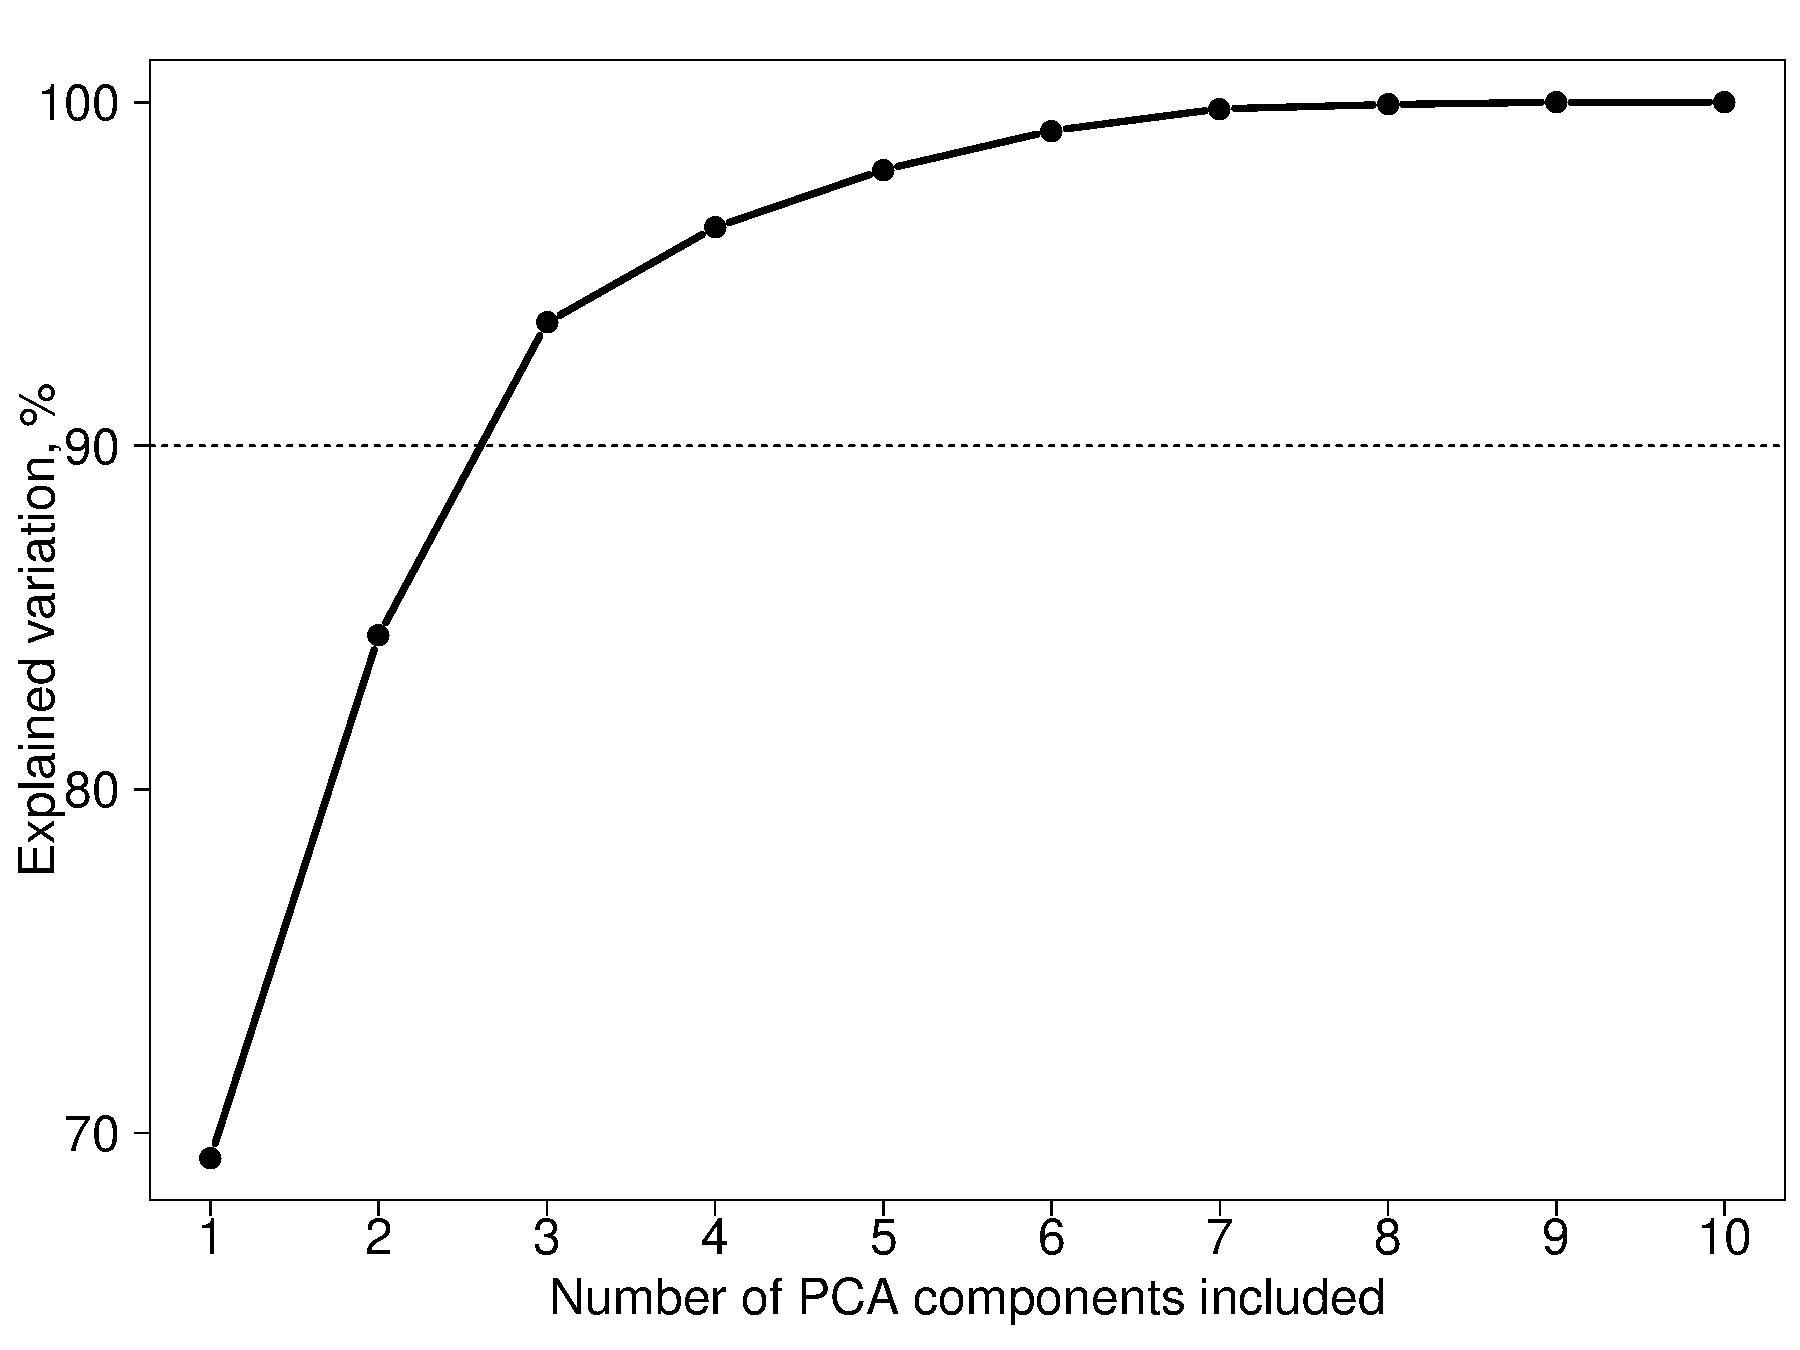
\includegraphics[width = 0.99\textwidth]{PCA_Variation.pdf}
  \end{minipage} \hfill
  \begin{minipage}{0.49\textwidth}
    b)\\
    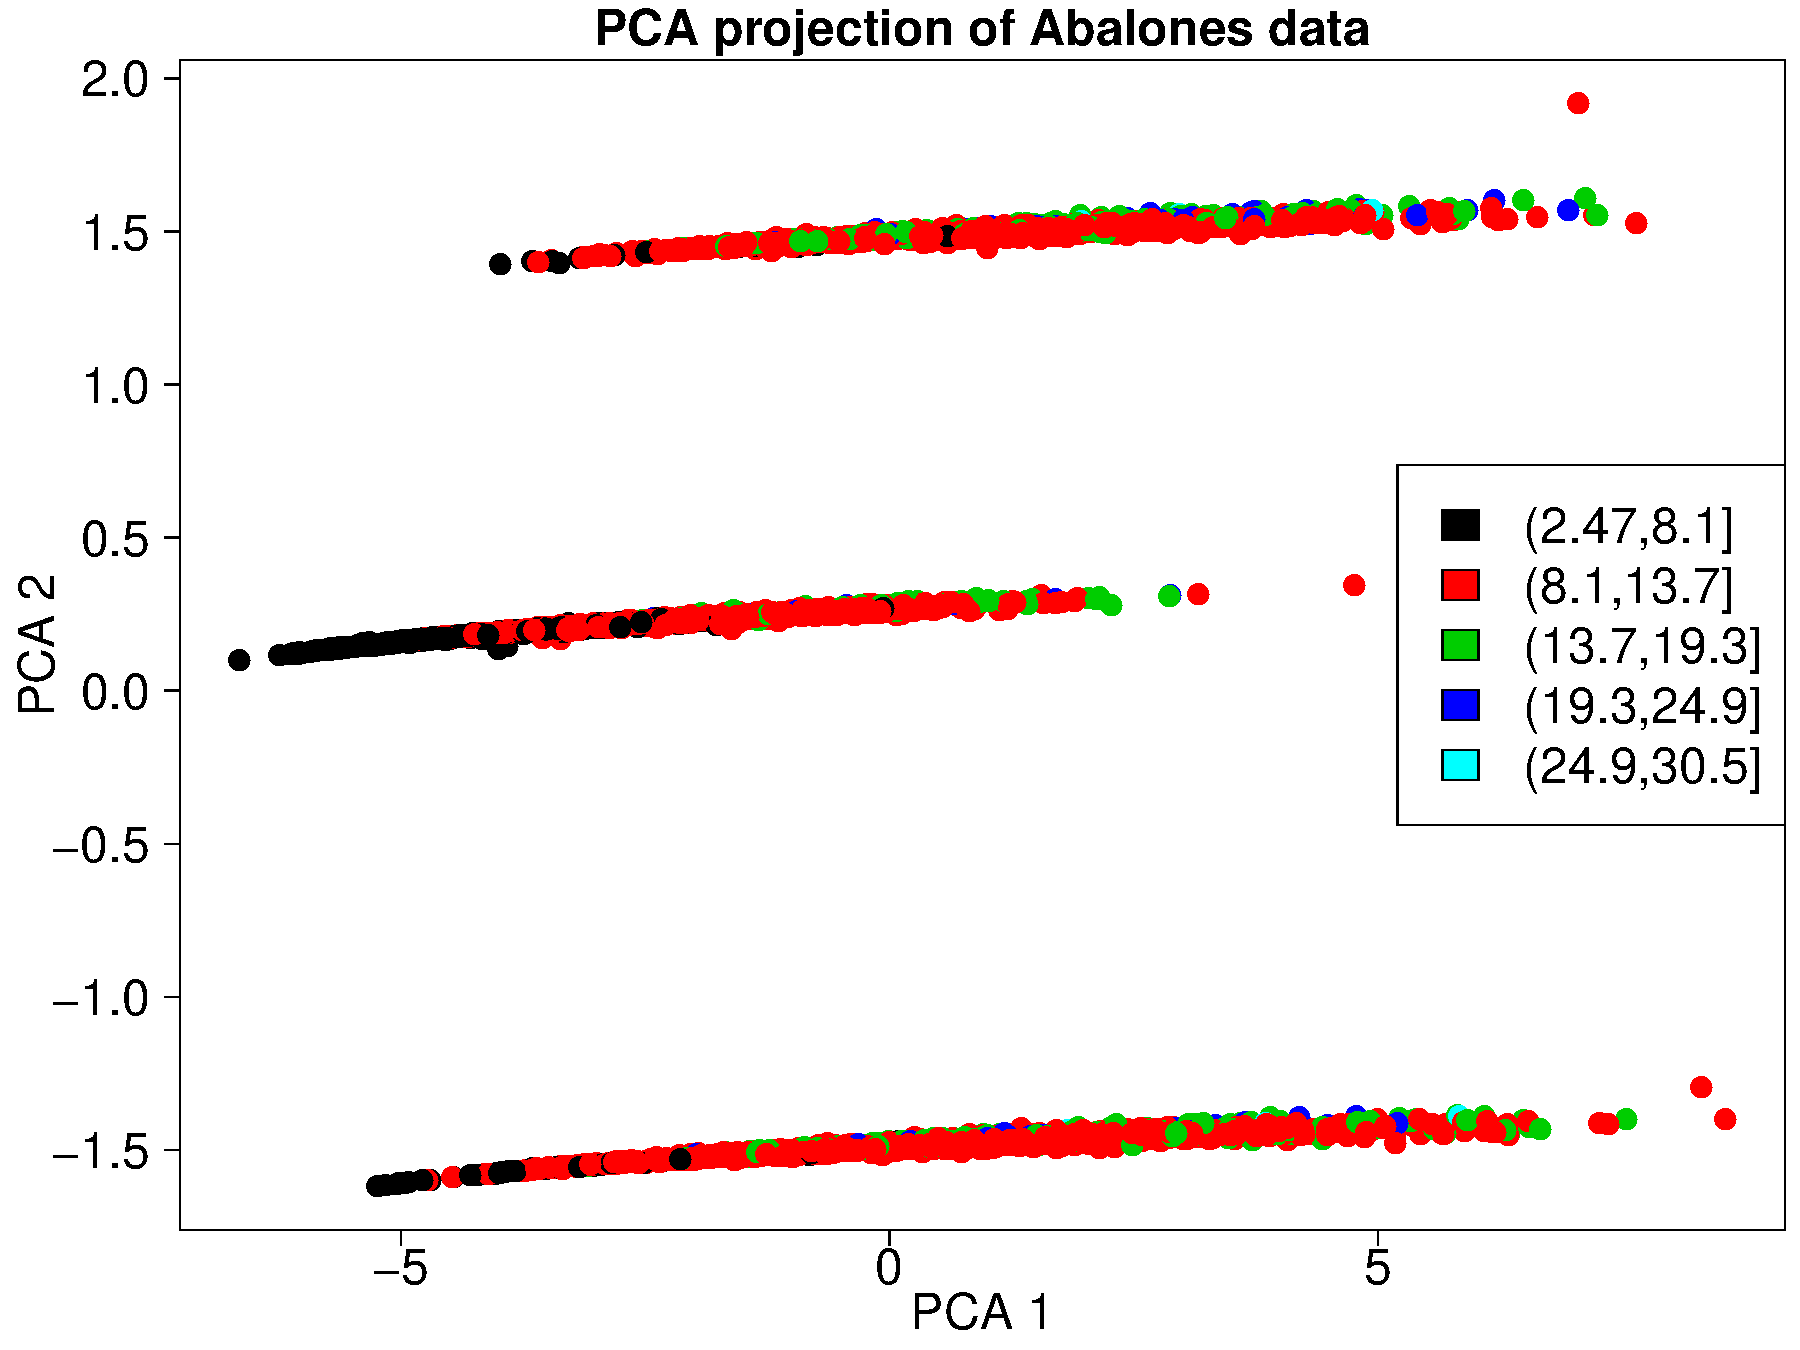
\includegraphics[width = 0.99\textwidth]{PCA_Projection.pdf}
  \end{minipage} \vfill
  \caption{a) The amount of explained variation as a function of the number of
    PCA components included.  The first two principal components explain around
    85 \% variation in the data. b) PCA projection of Abalones data to the first
    two principal components, points colored according to the age range they
    belong to.  Coloring of points is kept consistent throughout the report.}
  \label{fig:pca}
\end{figure}

\subsection{Gaussian Mixture Model}
A mixture model is a probabilistic model for representing the presence of
subpopulations within an overall population, without requiring that an observed
data set should identify the sub-population to which an individual observation
belongs.  A gaussian mixture model (GMM) uses k multivariate Gaussians to model
the data, and each of the gaussians is given a mixture coefficient.  With GMM,
the primary goal is to find out the optimal number of clusters to use in the
model.  This can be achieved in the following ways.  On the outer level, the
number of clusters in the model (with minimum of two clusters) is chosen and the
Bayesian Information Criteria (BIC = -2$\log$L + p $\log$N) or Akaike's
Information Criteria (AIC = -2$\log$L + 2p) are calculated (L is the log
likelihood of observing the data, p is the number of parameters in the model,
and N is the number of observations), and on the inner level the evaluation
cross-validation error (CVE) is calculated.

Prior to clustering, we standartized the data (subtract the mean and divide over
standard deviation attribute-wise).  To prevent the potential convergence
problems of the EM-algorithm for the GMM due to shrinking variance, we first ran
PCA before fitting the GMM.  In theory, that should decorrelate the features as
much as possible and make the problem of shrinking variances go away.  In
reality, our analysis showed that the more components are included into GMM the
better, and there is no optimal value for the number of components in the GMM
model.  We limited ourselves to up to 20 clusters with 5-fold cross-validation.
The results are presented in Fig.~\ref{fig:gmm}a.  Both the BIC and AIC
information criteria and the CVE keep decreasing with the increasing number of
components in the model, and there is no optimal value for it.  Nevertheless,
since there are actually 5 age ranges and therefore 5 clusters in the group, we
can look into fitting a GMM model with k = 5 components to the data.  The model
is visualized in Fig.~\ref{fig:gmm}b.  The cluster each observation is assigned
to is indicated by the color of the circle around the point, and each inner
color corresponds to the true age range of the points in Fig.~\ref{fig:pca}b.
The grey cluster mainly comprises the black and the red abalones, which means
the younger ones ([2.47 - 13.7) years).  The yellow cluster comprises mostly
  only the black points, which means the youngest abalones ([2.47 - 8.1) years).
    There are mixtures of all ages in the pink cluster, and the cyan and the
    blue cluster have a substantial amount of older abalones.

\begin{figure}[h!]
  \begin{minipage}{0.49\textwidth}
    a)\\
    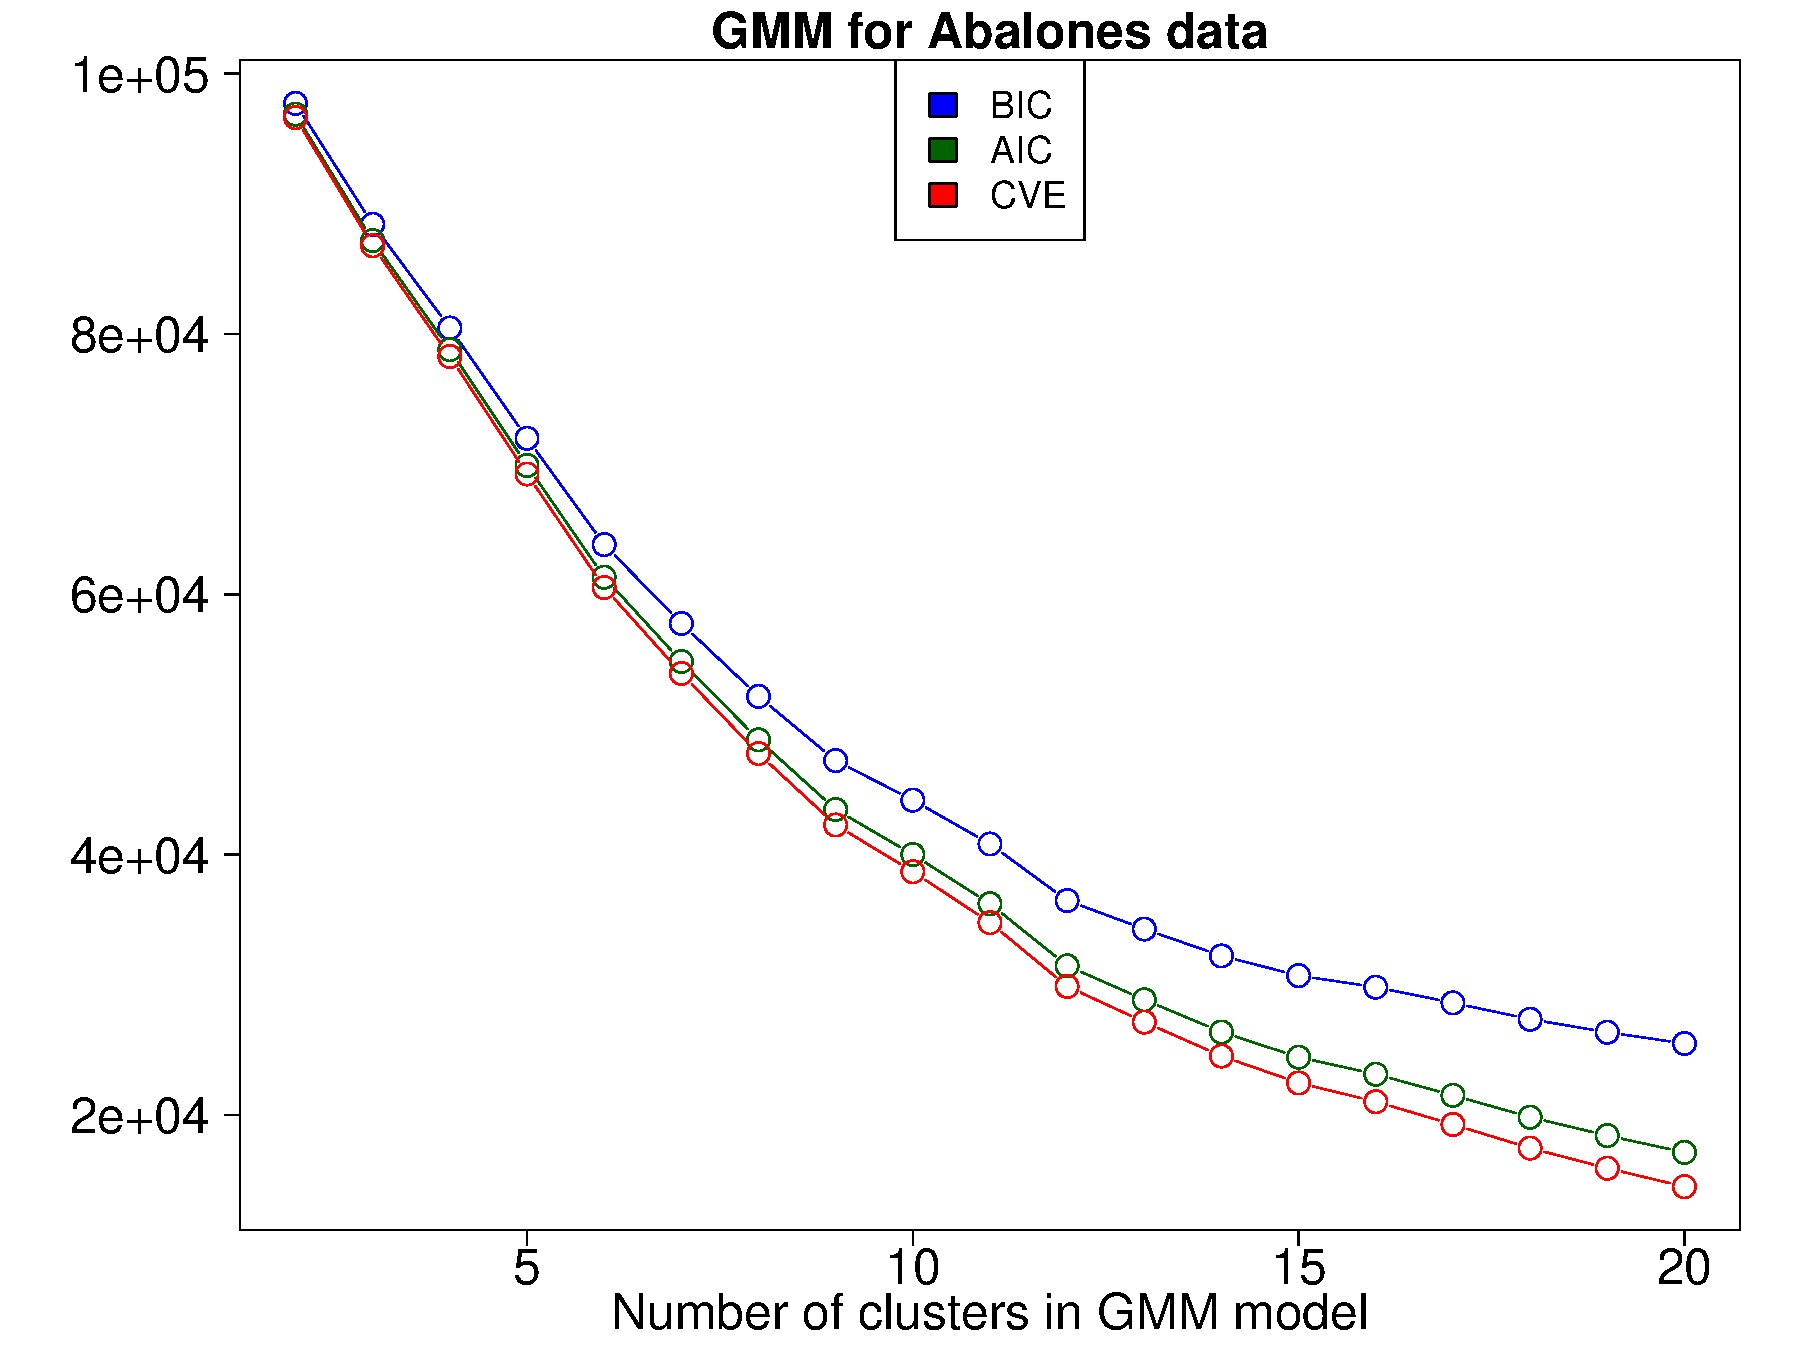
\includegraphics[width = 0.99\textwidth]{GMMCV1.pdf}
  \end{minipage} \hfill
  \begin{minipage}{0.49\textwidth}
    b)\\
    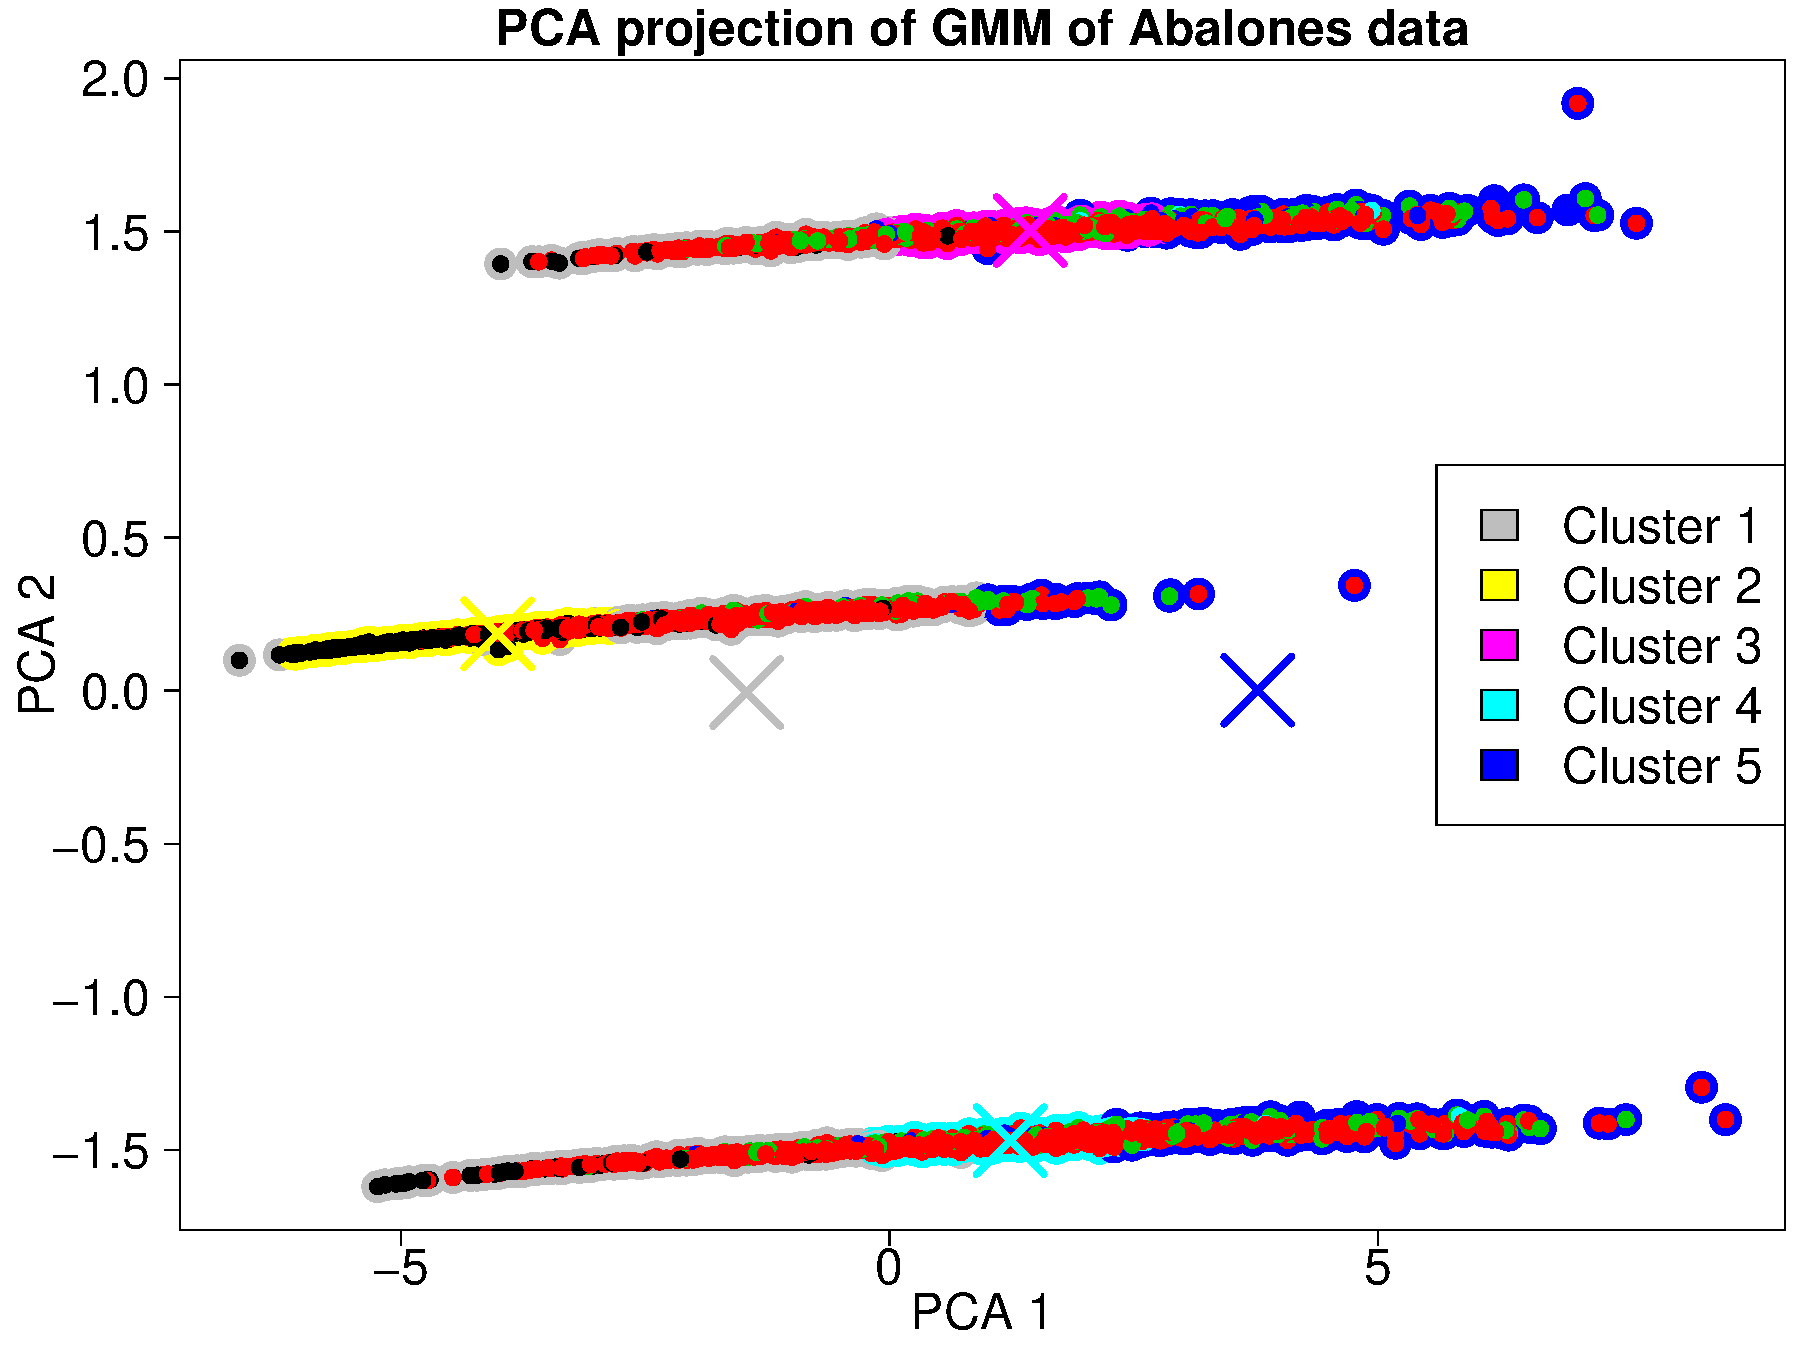
\includegraphics[width = 0.99\textwidth]{GMM_data.pdf}
  \end{minipage} \vfill
  \caption{a) Detecting the optimal number of clusters with the help of GMM
    model.  We used up to 20 clusters with 5-fold cross-validation, but found no
    optimal value of the components in the model.  b) Visualization of GMM model
    with 5 components fitted to the data on the first two PCA components.  The
    cluster each observation is assigned to is indicated by the color of the
    circle around the point, and each inner color corresponds to the true age
    range of the points in Fig.~\ref{fig:pca}b.}
  \label{fig:gmm}
\end{figure}

\subsection{Hierarchical clustering}
Hierarchical clustering is a method of cluster analysis which seeks to build a
hierarchy of clusters.  The agglomerative strategy for hierarchical clustering
(HCA) is a ``bottom up'' approach --- each observation starts in its own
cluster, and pairs of clusters are merged as one moves up the hierarchy.  At
some point, all observations are assigned to the same single cluster at the top
of the dendrogram.  We were not able to evaluate the optimal number of clusters
in the model using the GMM, but using the same logic as above we can think of
cutting the dendrogram so that it produces 5 clusters.

The results are presented in Fig.~\ref{fig:hclust}.  We fitted the hierarchial
clustering model to the data using the euclidean dissimilarity measure and the
Ward's linkage function.  The dendrogram is presented in Fig.~\ref{fig:hclust}a,
where the colored rectangles represent the clusters after the dendrogram was cut
into 5 of them.  In Fig.~\ref{fig:hclust}b, the HCA model is visualized in the
same way as in Fig.~\ref{fig:gmm}b.  Same as for Fig.~\ref{fig:gmm}b, the grey
and the yellow classes represent mostly the younger abalones, and pink cyan and
blue clusters contain more of the older abalones.

\begin{figure}[h!]
  \begin{minipage}{0.49\textwidth}
    a)\\
    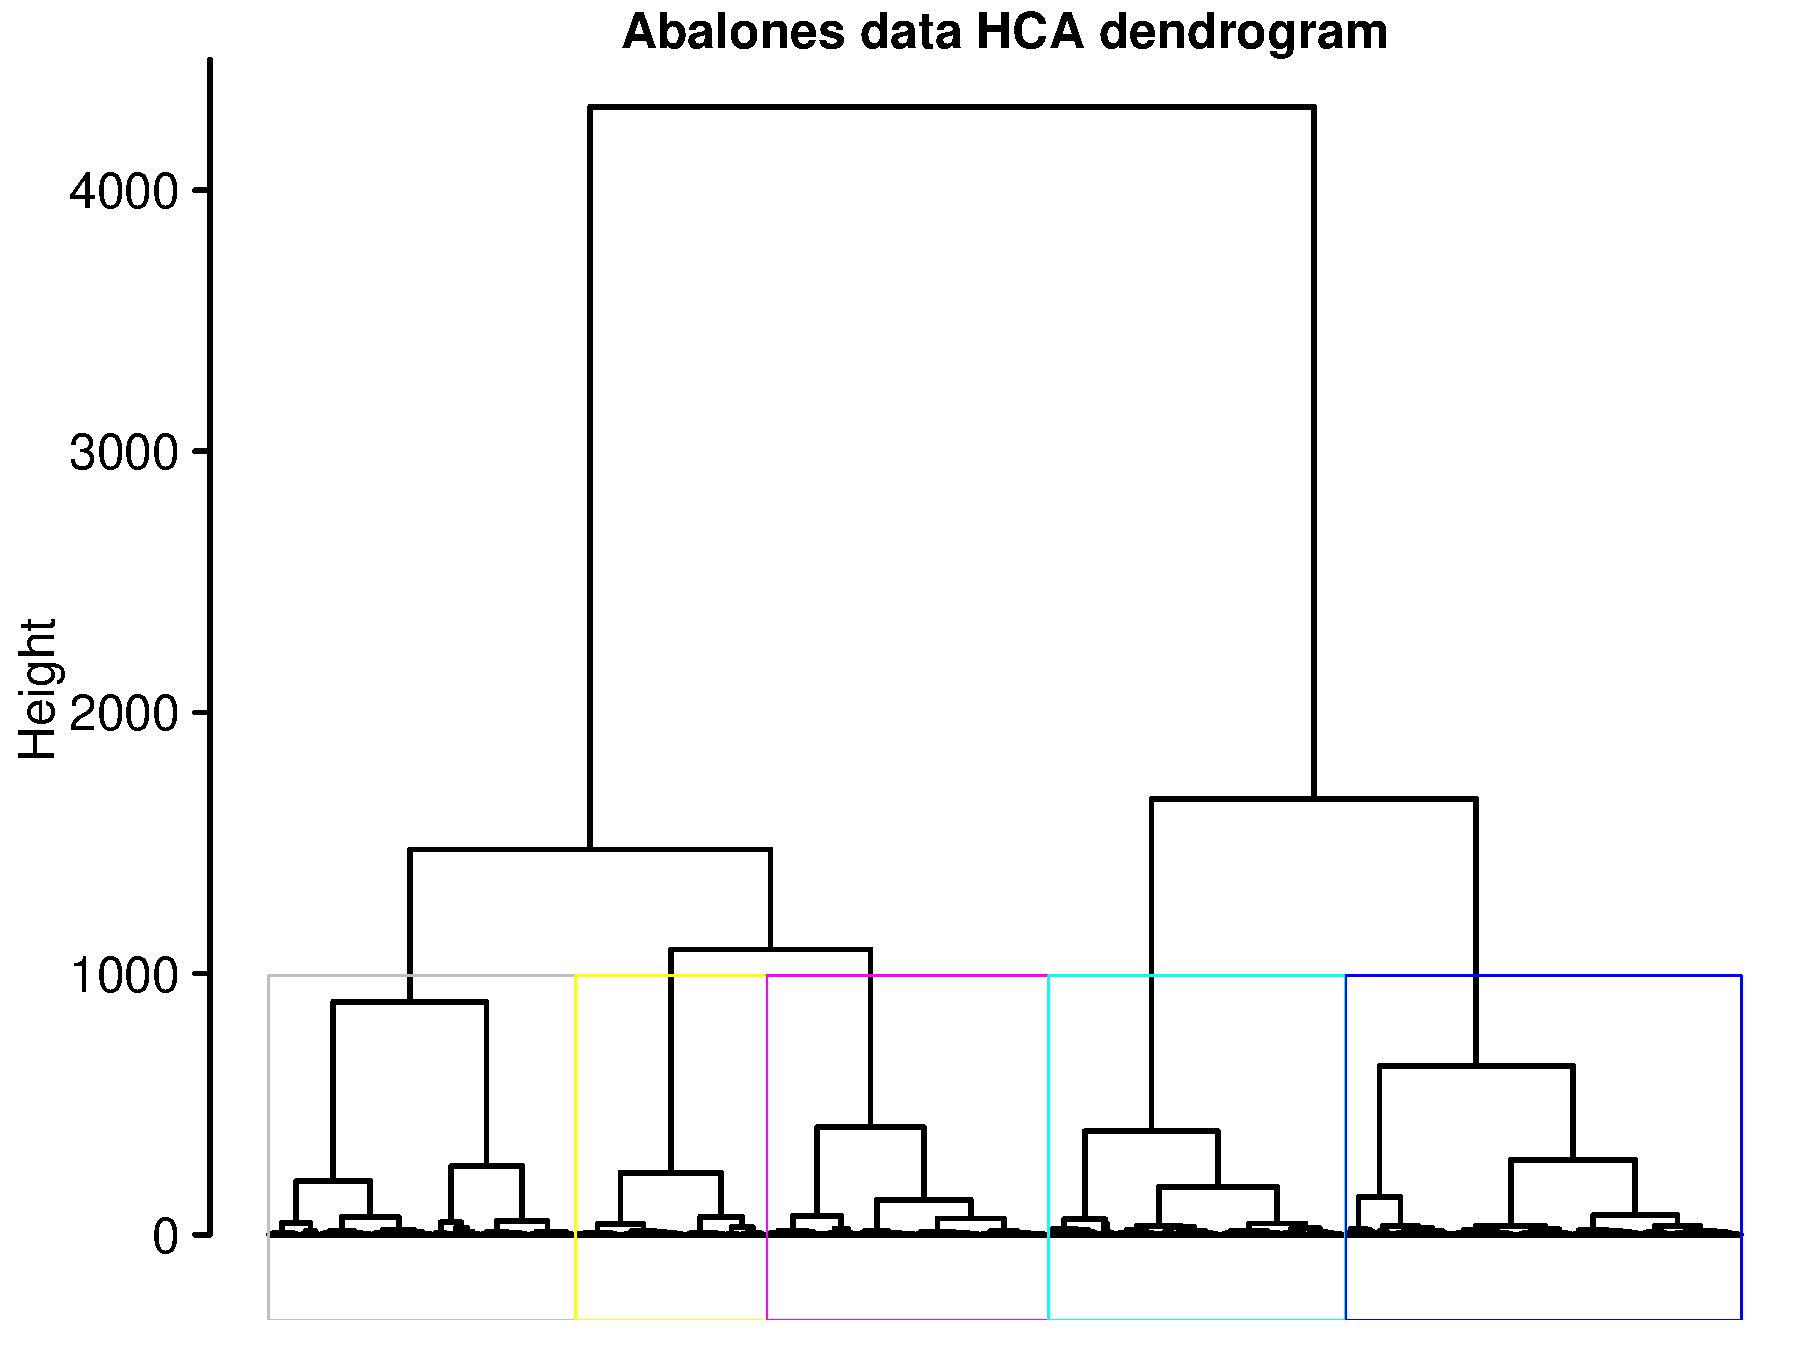
\includegraphics[width = 0.99\textwidth]{HClust_dendrogram.pdf}
  \end{minipage} \hfill
  \begin{minipage}{0.49\textwidth}
    b)\\
    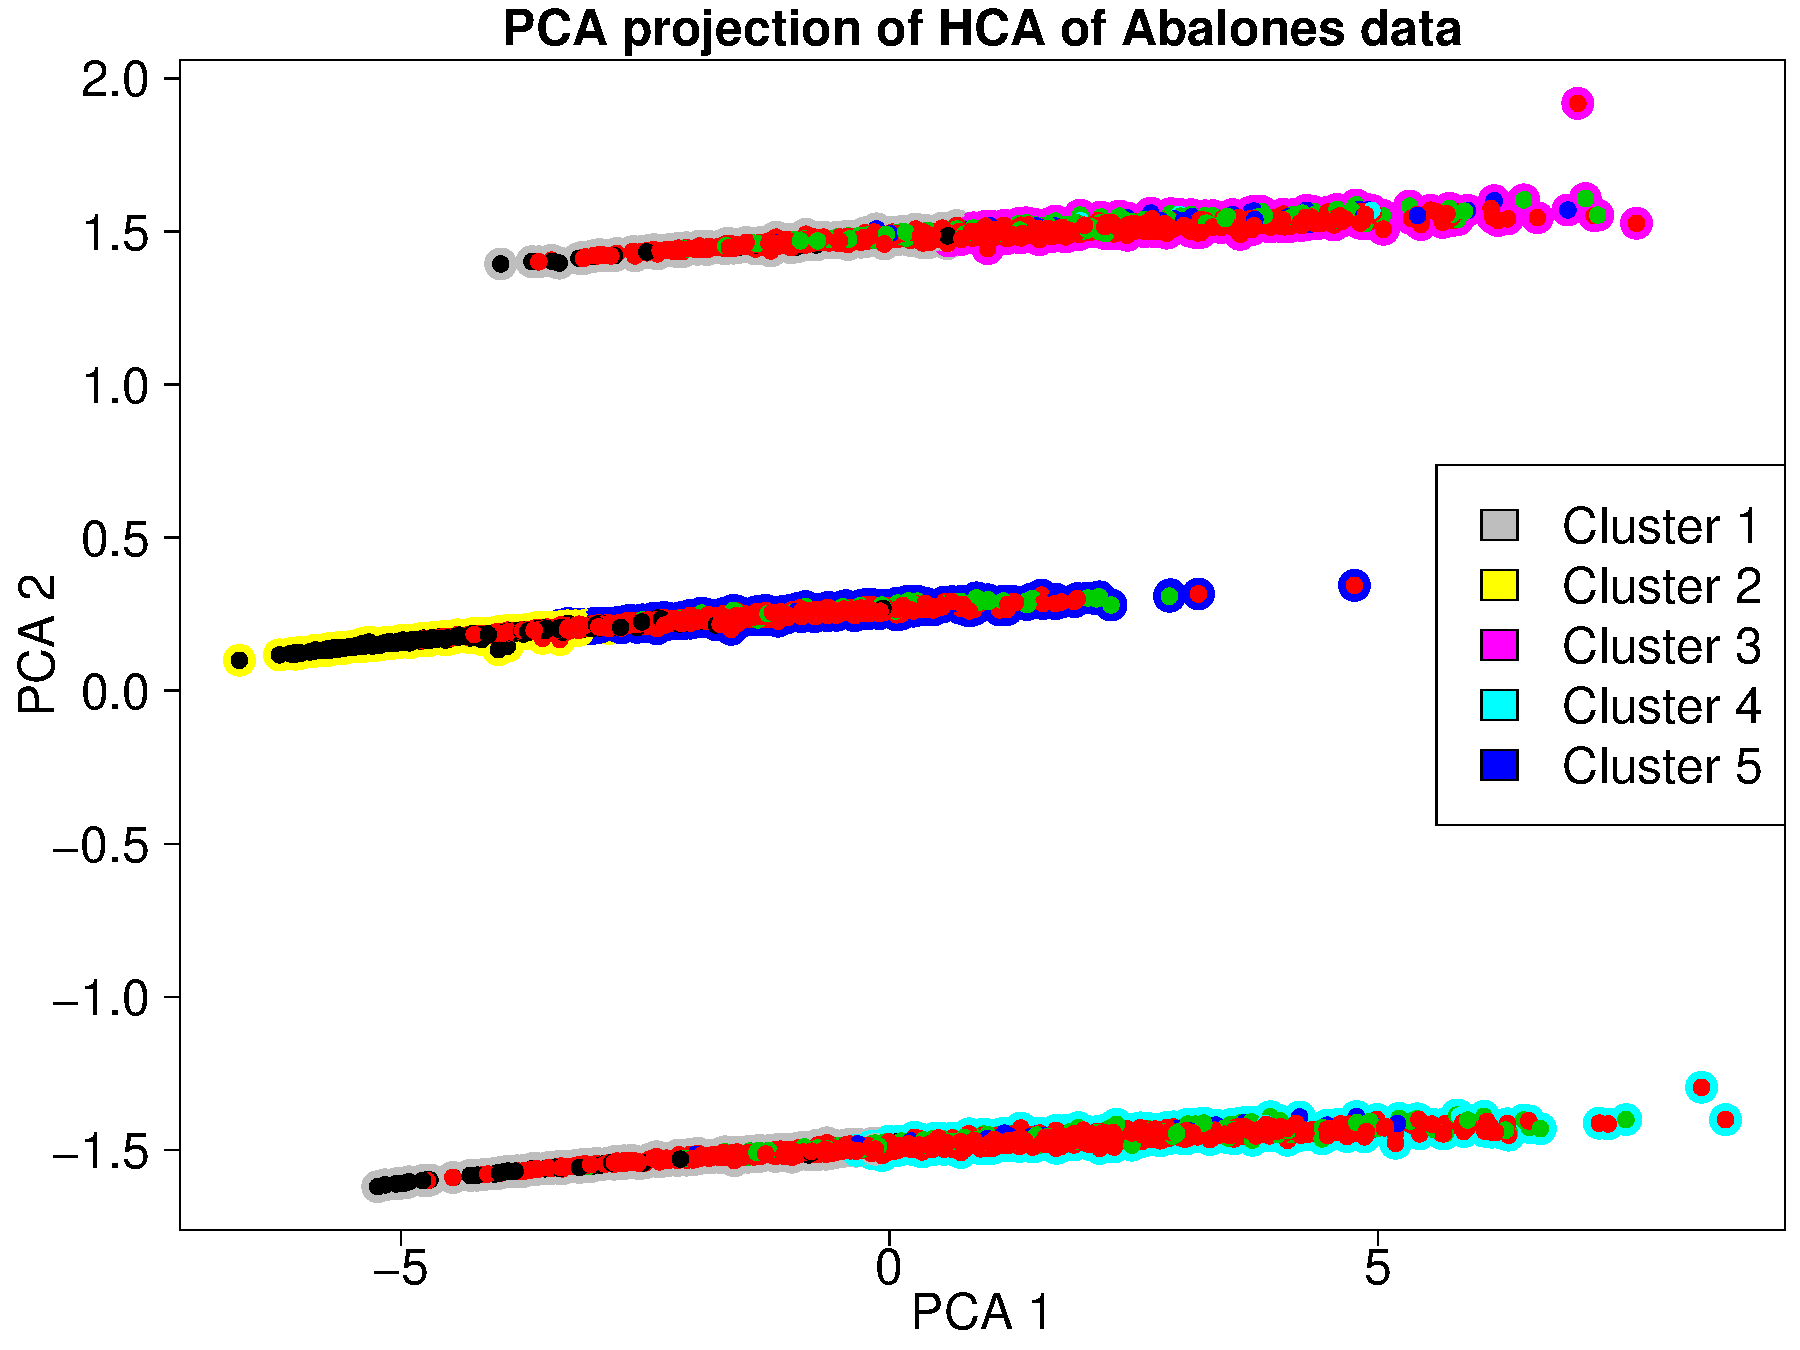
\includegraphics[width = 0.99\textwidth]{HClust_data.pdf}
  \end{minipage} \vfill
  \caption{a) The dendrogram of the HCA model fitted to the abalones data using
    the euclidean dissimilarity measure and the Ward's linkage function.
    Colored rectangles represent the five clusters after the dendrogram was cut
    into five pieces.  b) Visualization of HCA model fitted to the data on the
    first two PCA components, similar to Fig.~\ref{fig:gmm}b.}
  \label{fig:hclust}
\end{figure}

\subsection{Evaluation of the quality of clustering}
For the hierarchial clustering, we can consider several measures of cluster
validity (Entropy, Purity measures of cluster purity and Rand and Jaccard binary
similarity measures) and how they behave when cutting the dendrogram at
different levels.  The result is presented in Fig.~\ref{fig:clust_quality}a.  We
see that the Purity measure is saturated already when using a single cluster in
the HCA model, Rand is saturated after the two clusters in the model, and
Entropy and Jaccard measures decrease slightly with the increase of number of
clusters in the model.

We can also compare the two models --- GMM and HCA, cut at the same number of
clusters as the GMM in terms of the abovementioned cluster validity measures,
and this result is presented in Fig.~\ref{fig:clust_quality}.  The figure
suggests that there is simply no difference in any of the cluster validity
measures obtained by different methods.

\begin{figure}[h!]
  \begin{minipage}{0.49\textwidth}
    a)\\
    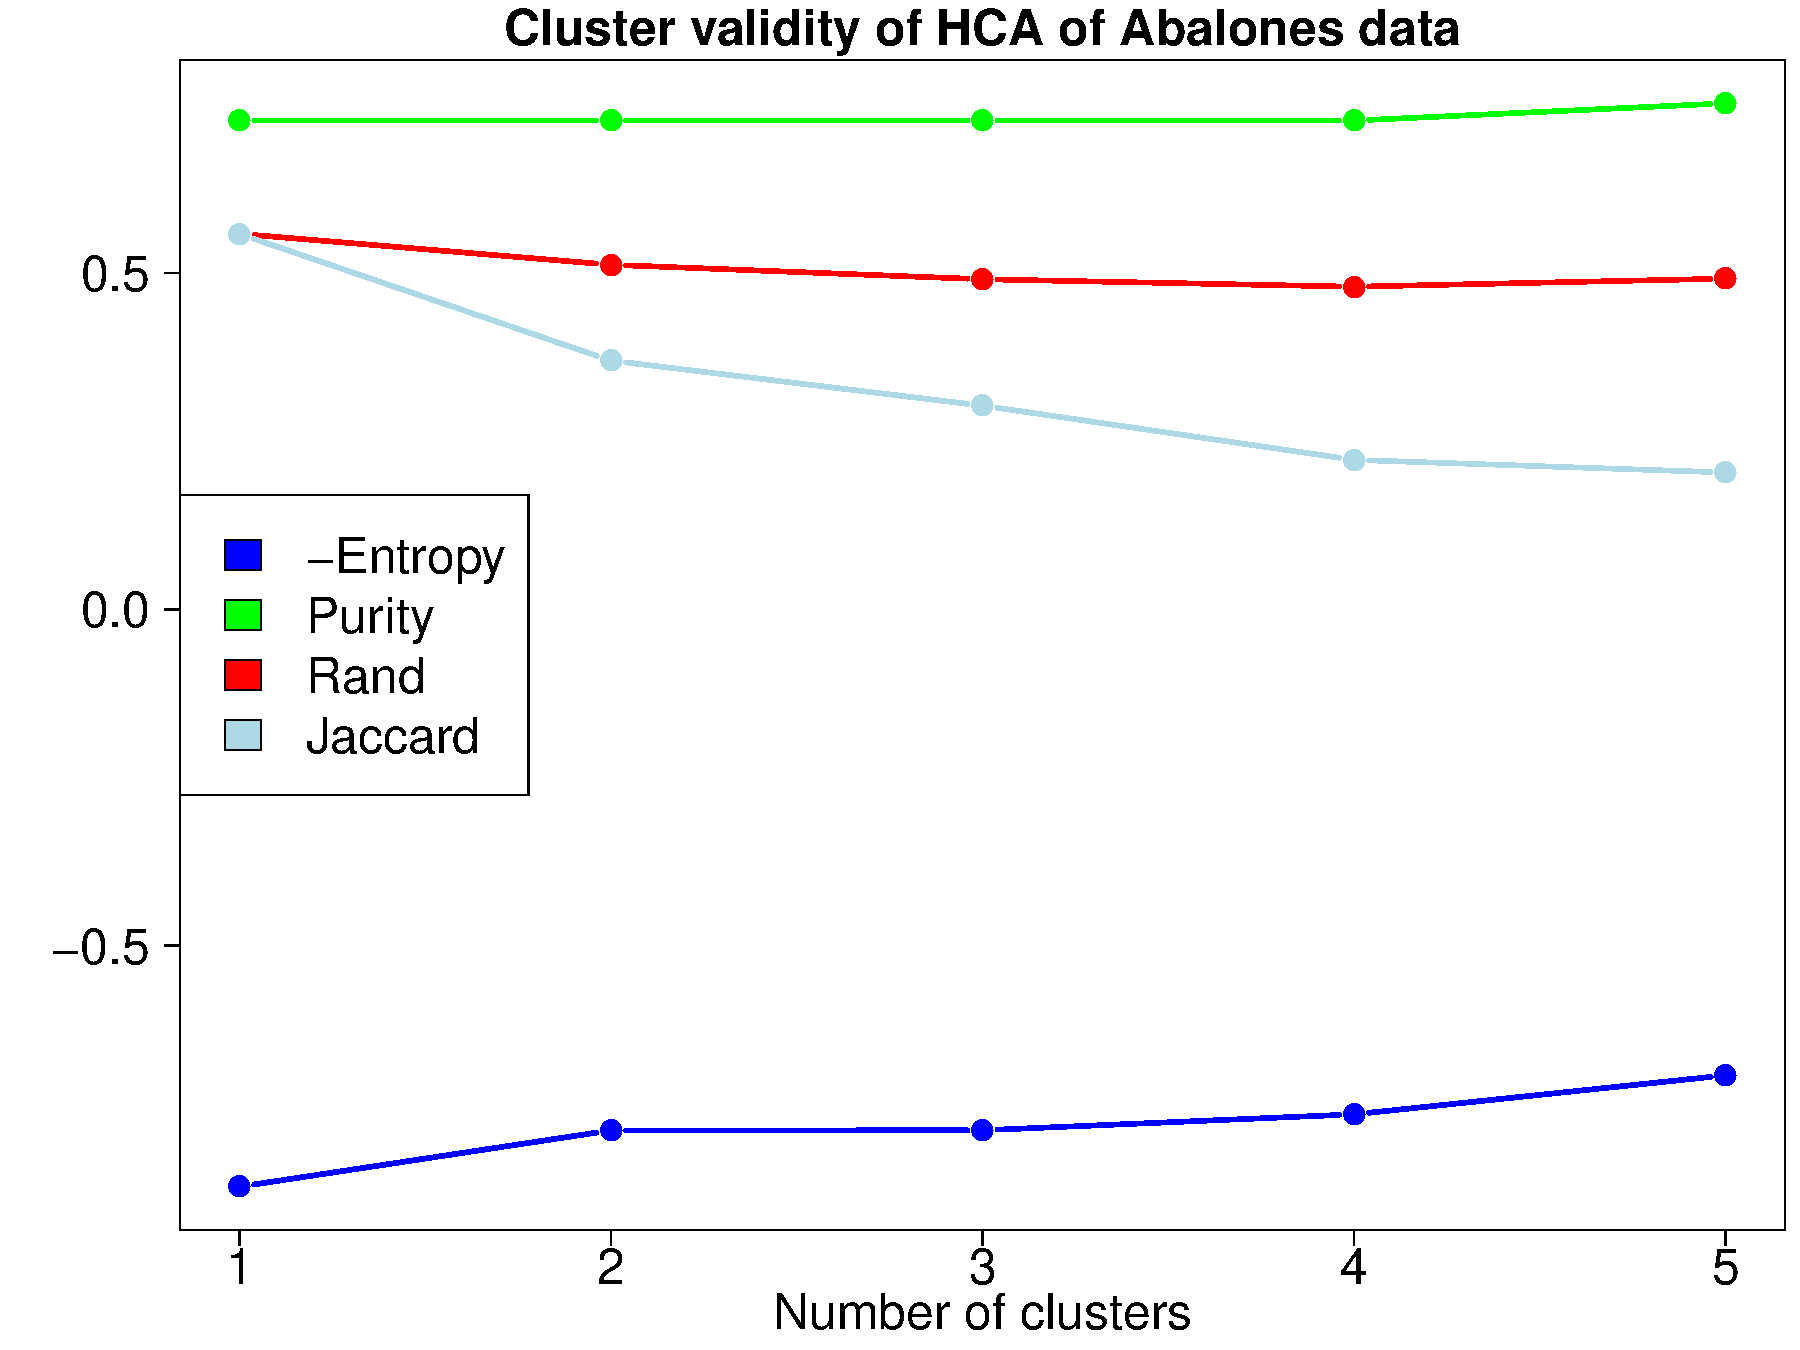
\includegraphics[width = 0.99\textwidth]{HClust_validity.pdf}
  \end{minipage} \hfill
  \begin{minipage}{0.49\textwidth}
    b)\\
    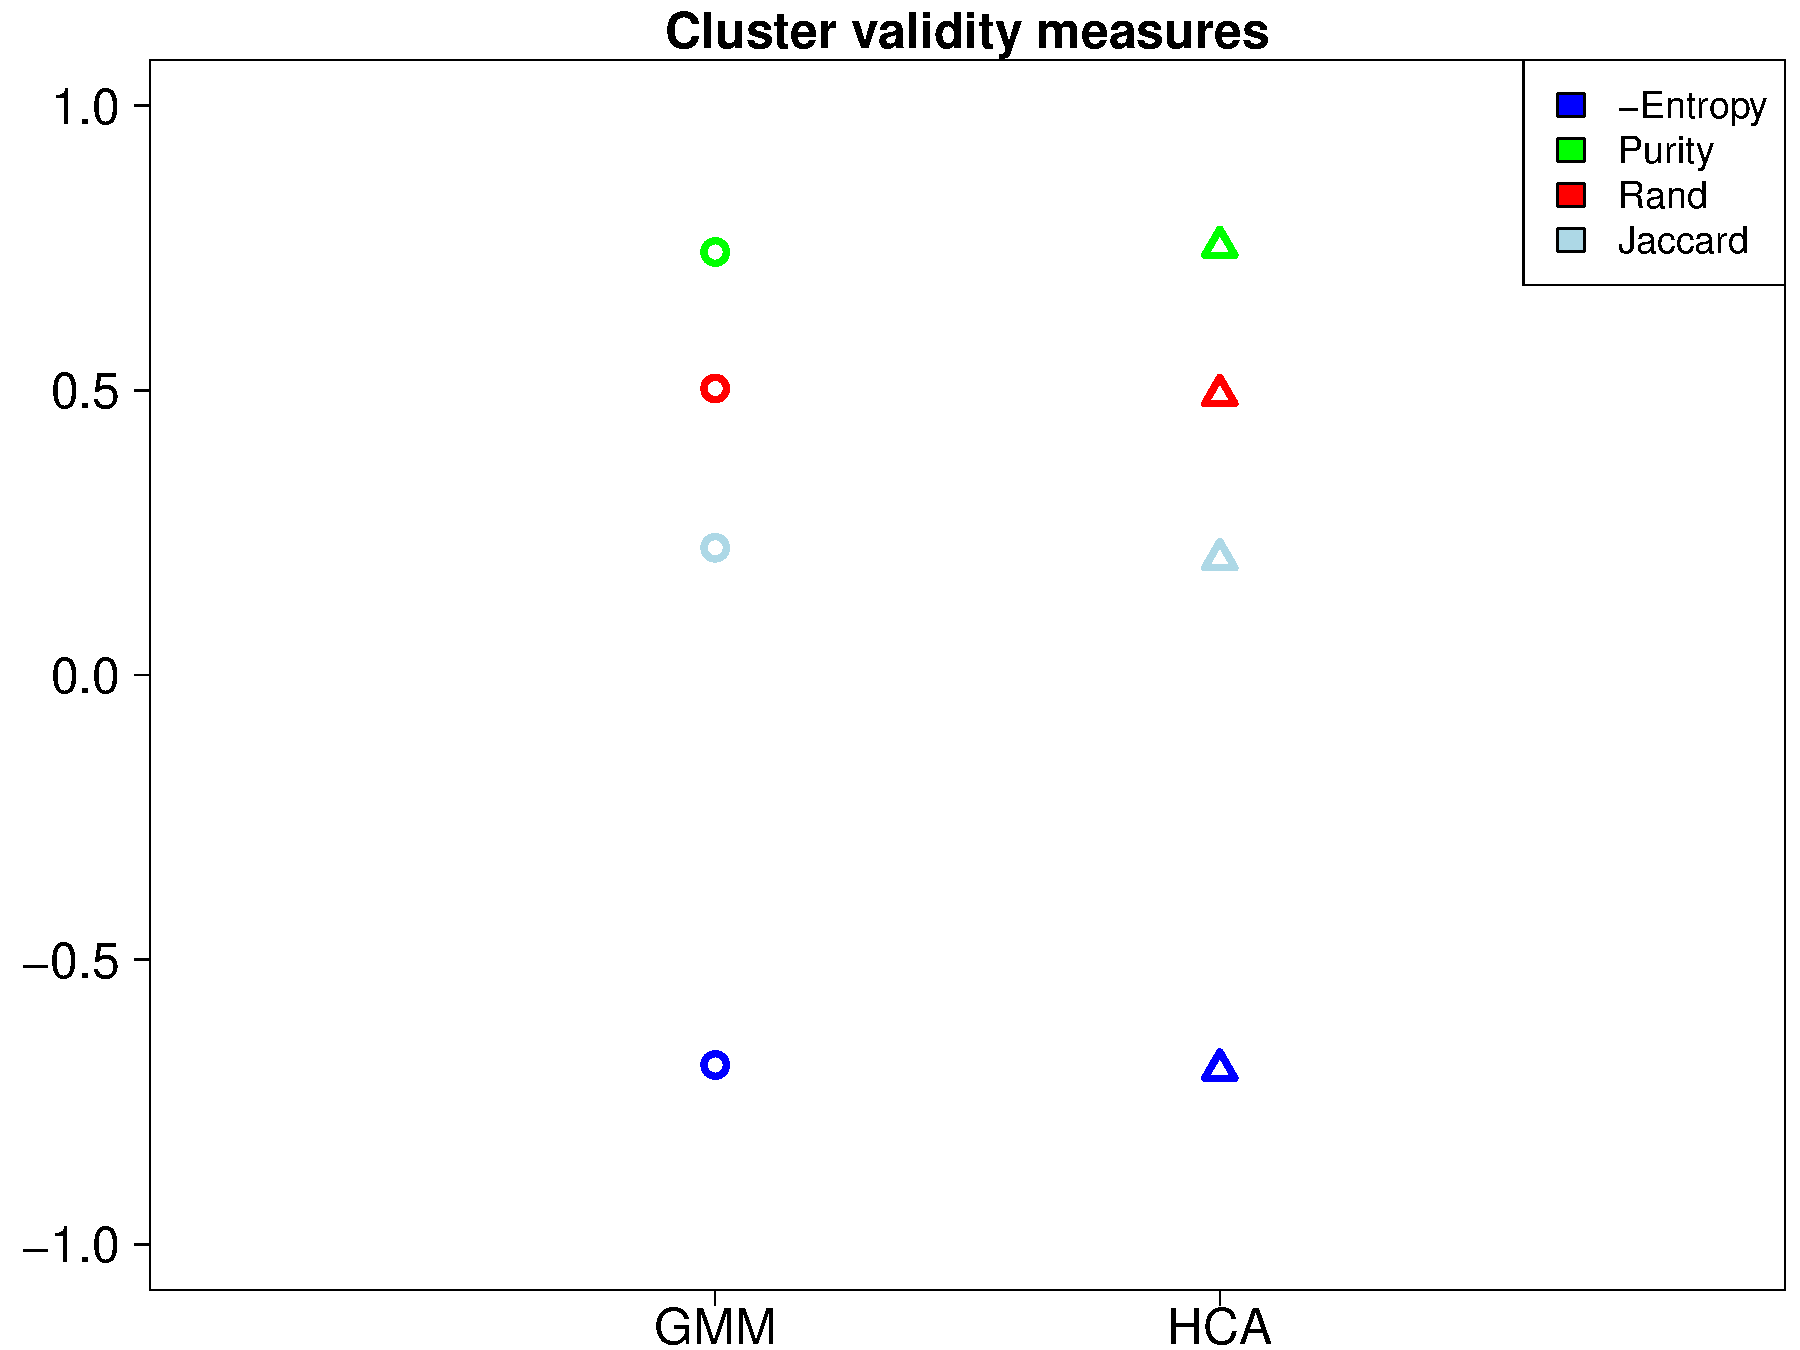
\includegraphics[width = 0.99\textwidth]{Cluster_comparison.pdf}
  \end{minipage} \vfill
  \caption{a) Measures of cluster validity as a function of the number of
    cluster in the HCA model.  b) Comparison of GMM and HCA models in terms of
    cluster validity measures.}
  \label{fig:clust_quality}
\end{figure}

\newpage
%%%%%%%%%%%%%%%%%%%% Association mining
\section{Association mining}
\label{sec:association}
\subsection{Apriori algorithm}
Prior to using the association mining, first the data have to be expressed in a binary format. The binarization of the Abalone data was made using the following criteria: The continuous attributes were binarized by their median value and the factor attributes were binarized by each one of their factors. After the binarization, we can define $I=\{i_1, i_2,\ldots , i_d\}$ as the set of all attributes and $T=\{t_1, t_2, \ldots ,i_N\}$ as the set of all transactions (each data observation). Each transaction $t_i$ contains a subset of items chosen from $I$. With the above definitions it is possible to define Association rules. An association rule (AR) is an implication expression of the form $X \rightarrow Y$, where $X$ and $Y$ are disjoint itemsets. The strength of an association rule can be measured in terms of its support and confidence. Support determines how often a rule is applicable to a given data set, while confidence determines how frequently items in $Y$ appears in transactions that contain $X$.

With the support and confidence, the association rule mining problem can be decompose in two major subtasks: 1) Find all the item sets that satisfy a minimum value of support. These itemsets are called frequent itemsets. 2) Extract all high-confidence rules from the frequent itemsets found in the previous step. These rules are called strong rules.

Performing the subtasks is computational demanding, for that reason the $apriori$ principle is used. The $apriori$ principle says that \textit{if an itemset is frequent, then all of its subsets must also be frequent}. This reduce the number of candidate itemsets and the number of association rules to be compared.

The $apriori$ algorithm was implemented, results for the subtask number one on the Abalone data set with a minimum support of 65\% resulted in the following itemsets.
\begin{verbatim}
[1] "Apriori analysis done, extracting results"
$FreqItemSets
[1] "Age.H[Sup. 7e+01]"
\end{verbatim}

Results indicate that only the attribute Age.H (Age above the median) presents a support higher than 65\%. Then, the subtask number two was performed to explore the AR between Age.H and the rest of the attributes. Results for the AR with a minimum confidence of 65\% can be seen next.
\begin{verbatim}
$AssociationRules
[1] "Age.H <- [Conf. 7e+01,Sup. 7e+01]"            "VscrWght.H <- Age.H[Conf. 7e+01,Sup. 5e+01]" 
[3] "ShllWght.H <- Age.H[Conf. 7e+01,Sup. 5e+01]"  "ShckdWght.H <- Age.H[Conf. 7e+01,Sup. 4e+01]"
[5] "WhlWght.H <- Age.H[Conf. 7e+01,Sup. 5e+01]"   "Length.H <- Age.H[Conf. 7e+01,Sup. 5e+01]"   
[7] "Diameter.H <- Age.H[Conf. 7e+01,Sup. 5e+01]"  "Height.H <- Age.H[Conf. 7e+01,Sup. 5e+01]"
\end{verbatim}

\subsection{Association rules interpretation}
Exploring the association rules, we can see that the presence of Age higher than the median implies that there is higher probability for the Abalones to have higher viscera weight (VscrWght.H), shell wieght (ShllWght.H), Shucked weight (ShckdWght.H), Whole weight (WhlWght.H), length, diameter and height. Notice that there is not AR between the Age and Sex. This indicates that the Abalones age depends only on its physical characteristics an not on the Abalones sex. Finally, we conclude that the presence of the mentioned physical characteristics leads to higher Abalones age.


%%%%%%%%%%%%%%%%%%%% Outlier / Anomaly detection
\section{Outlier / Anomaly detection}
\label{sec:detection}
%% In this part of the exercise you should apply some of the scoring methods for
%% detecting outliers you learned in Exercise 11.  In particular, you should

%% \begin{enumerate}
%%   \item Rank all the observations in terms of the Gaussian Kernel density (using
%%     leave- one-out), KNN density, KNN average relative density and distance to
%%     Kth nearest neighbor for some suitable K. (If the scale of each attribute in
%%     your data are very different it may turn useful to normalize the data prior
%%     to the analysis).
%%   \item Discuss whether it seems there may be outliers in your data according to
%%     the four scoring methods.
%% \end{enumerate}

There exist two definitions of a data object as an outlier --- Hawkin's
definition (an outlier is an observation that differs so much from other
observations as to arouse suspicion that it was generated by a different
mechanism), and probabilistic definition (an outlier is an object that has a low
probability with respect to a probability distribution model of the data).
Inspection of outliers in the Abalones dataset is discussed below.

Prior to using the advanced methods of outlier detection, we show the recap of
the earlier results of descriptive data analysis.  The boxplots for each of the
standartized attributes are presented in
Fig.~\ref{fig:data_descriptive_analysis}a.  Boxplots define and display outliers
automatically, if the points fall outside the whiskers of the plot, and
according to the plot there are quite a number of outliers in each of the
attributes.  However, the boxplots do not reflect the original distribution of
the attributes, and that is given by their histograms presented in
Fig.~\ref{fig:data_descriptive_analysis}b.  The plot suggests that the outliers
in the boxplot are due to the skewed distributions of attributes, rather to any
anomally in them.  However, there are two points with abnormal heights, that are
definitely very suspicious.

\begin{figure}[h!]
  \begin{minipage}{0.49\textwidth}
    a)\\
    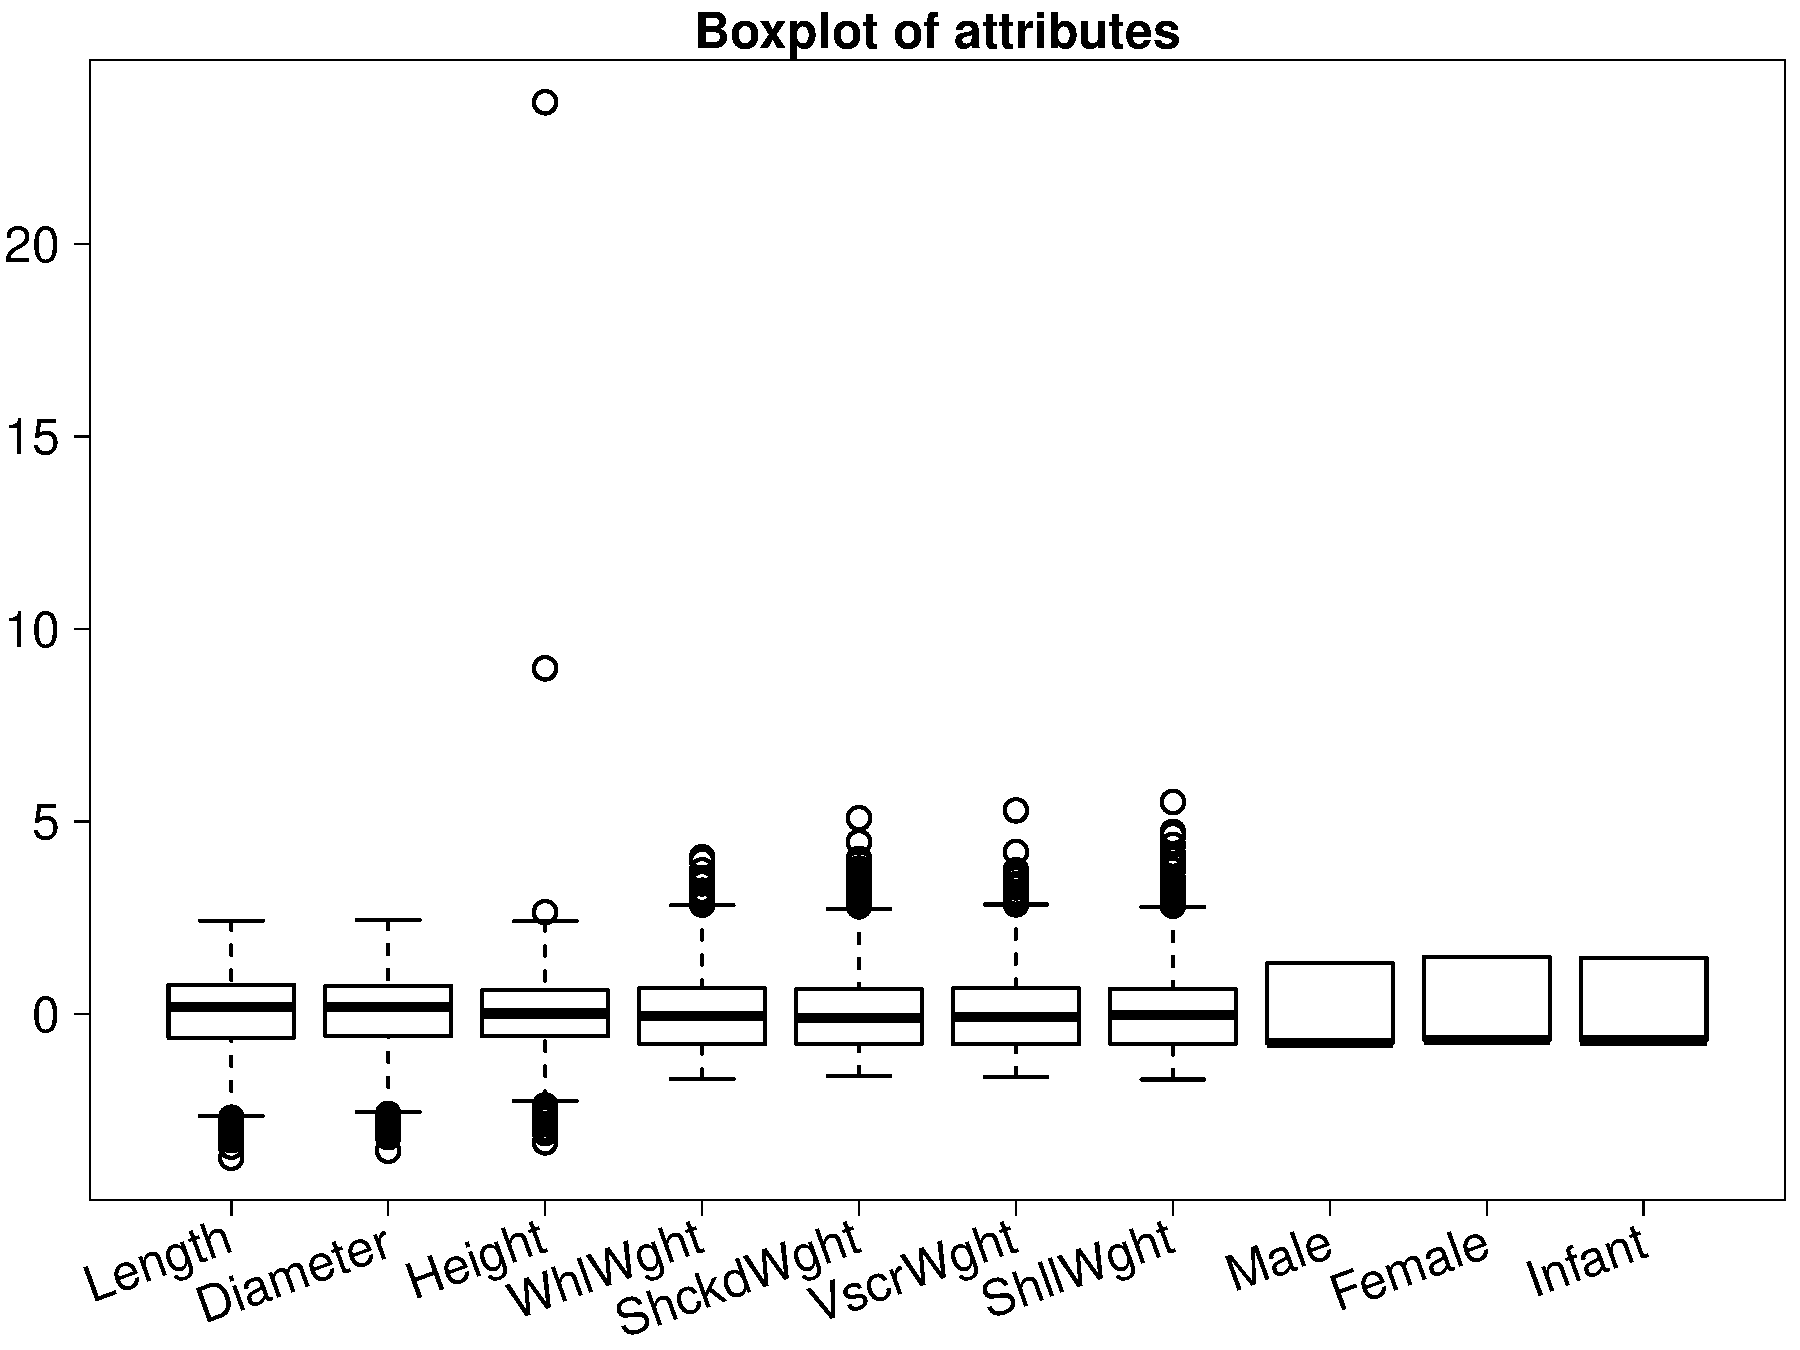
\includegraphics[width = 0.99\textwidth]{data_boxplot.pdf}
  \end{minipage} \hfill
  \begin{minipage}{0.49\textwidth}
    b)\\
    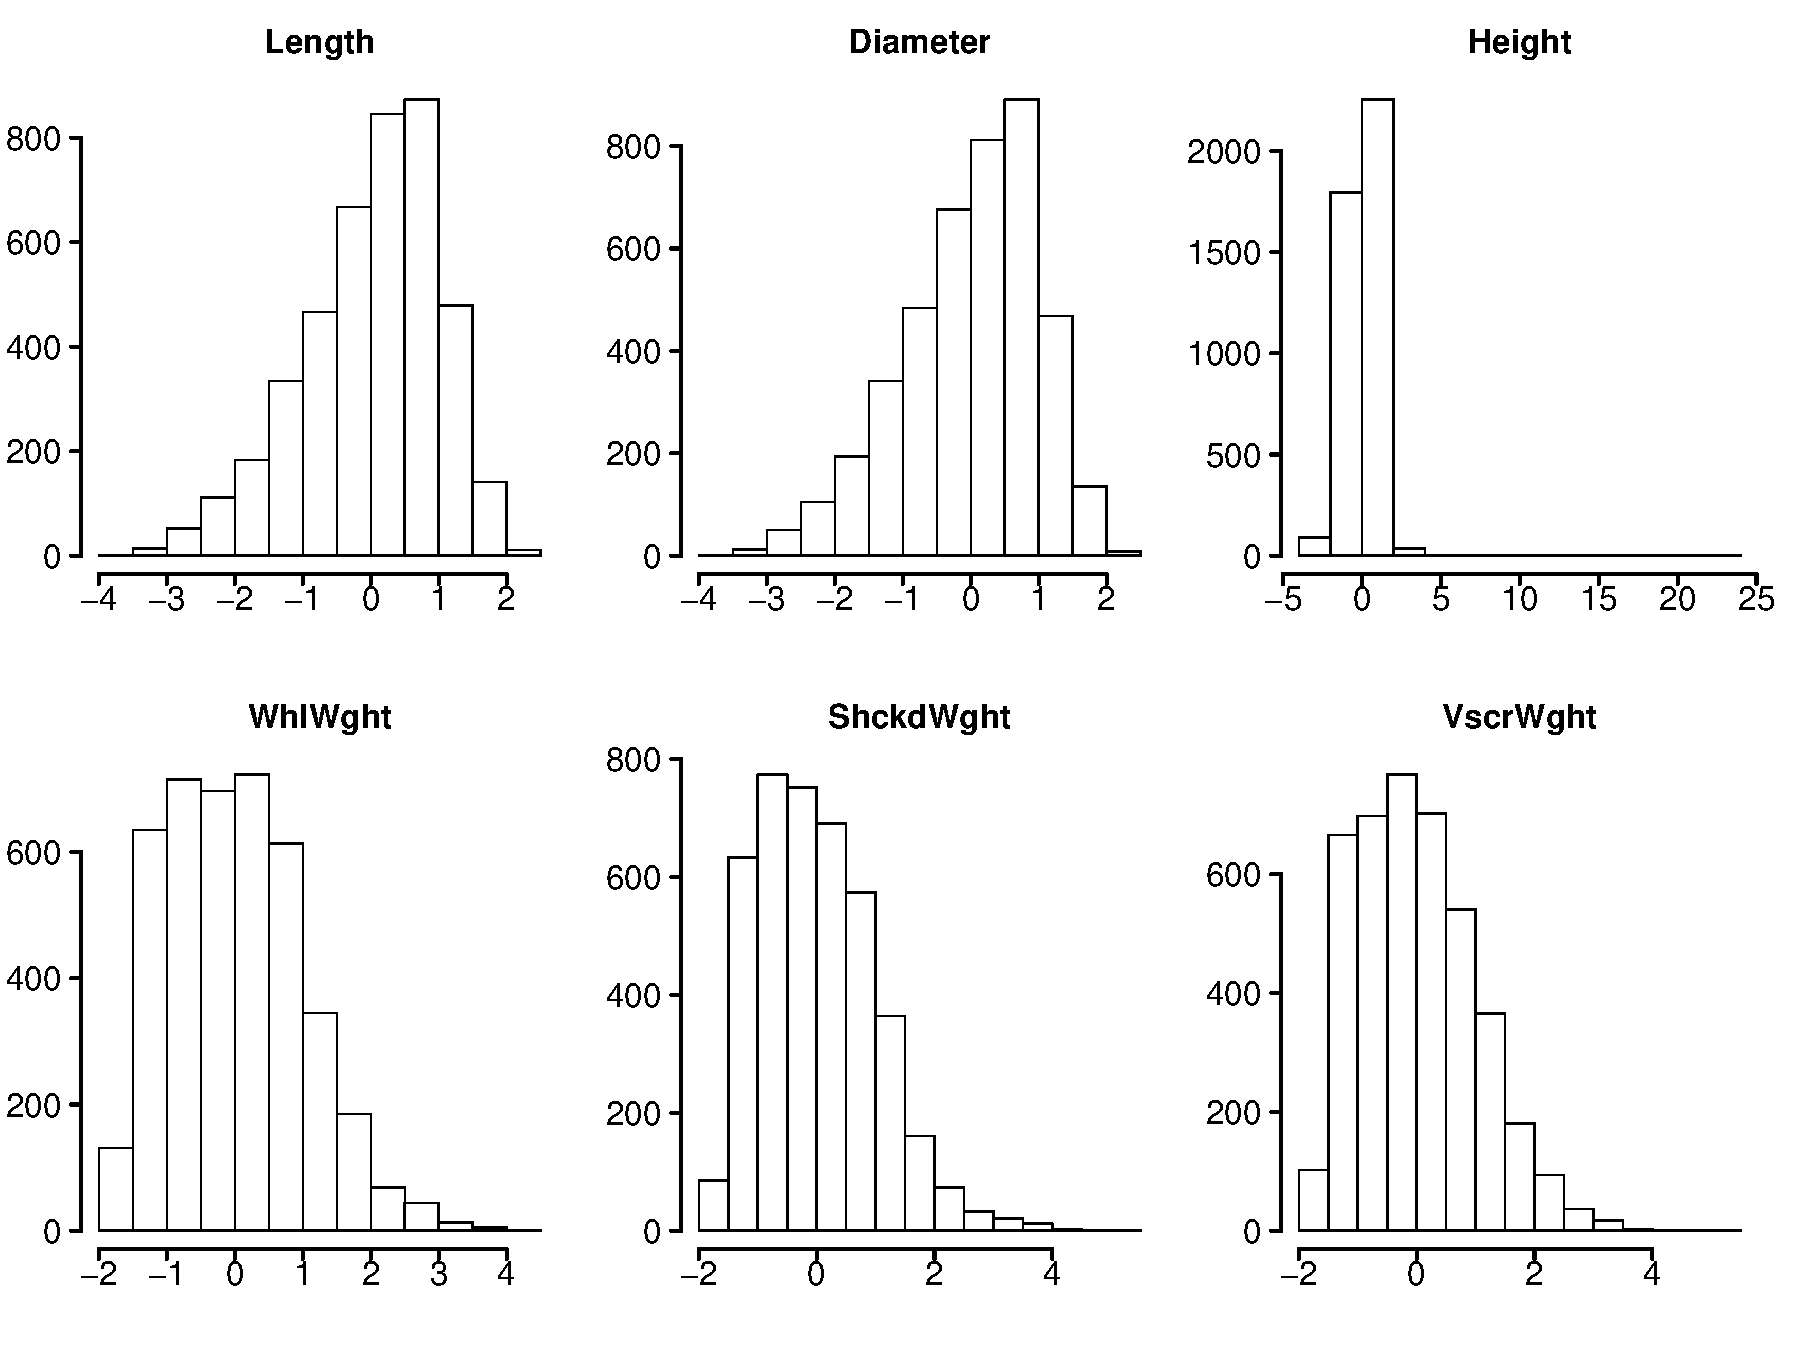
\includegraphics[width = 0.99\textwidth]{data_histogram.pdf}
  \end{minipage} \vfill
  \caption{a) Boxplot and b) histogram of standartized attributes of the
    Abalones dataset.}
  \label{fig:data_descriptive_analysis}
\end{figure}

An advanced method of outlier detection is to rank all observartions in the
dataset using a ranking system that reflects how abnormal the observation is.
The methods we applied were Gaussian Kernel density using leave-one-out
cross-validation (GKD), k nearest neighbors density (KNND), KNN average relative
density (KNNARD), and distance to k-th nearest neighbor (DKNN).  We tested
different values of the number of nearest neighbors k, but in the range from 5
to 30 it did not change the results significantly, so we ended up using k = 30.
Each of the methods ranked all observartions of the Abalones dataset in its own
way, and we selected the first 20 observations (i.e. 20 most suspicious ones)
and plotted their ranking score vs their index number in the dataset in
Fig.~\ref{fig:data_ranking}a.

\begin{figure}[h!]
  \begin{minipage}{0.99\textwidth}
    a)\\
    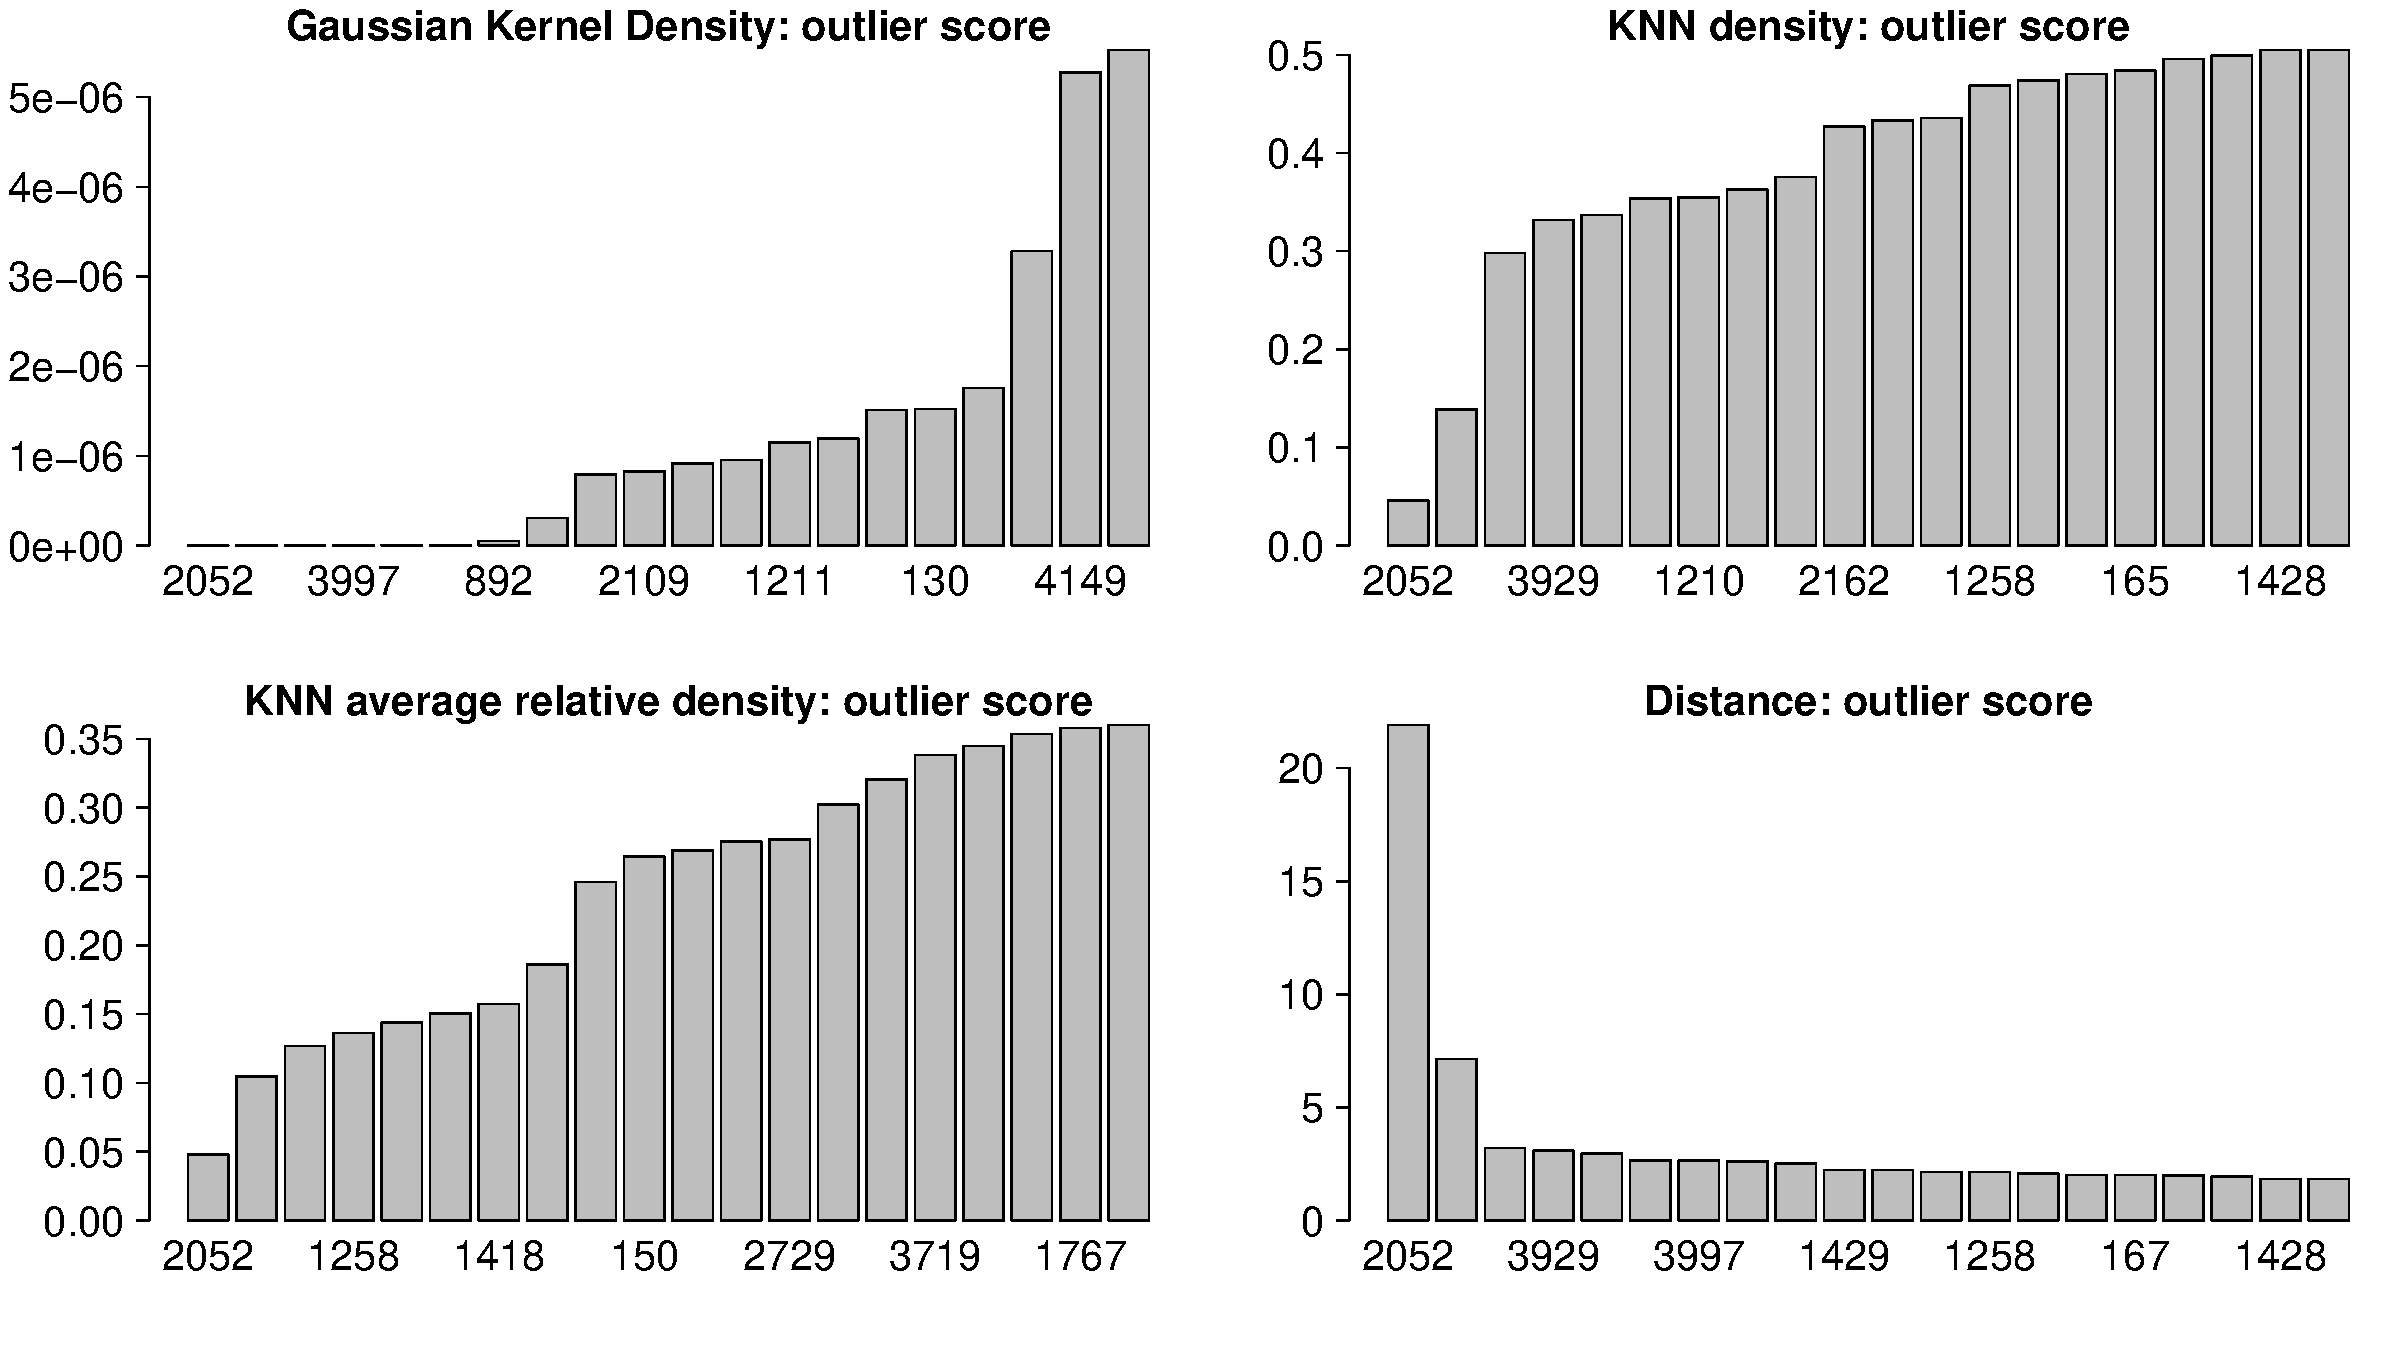
\includegraphics[width = 0.99\textwidth]{data_ranking.pdf}
  \end{minipage} \vfill
  \begin{minipage}{0.99\textwidth}
    b)\\
    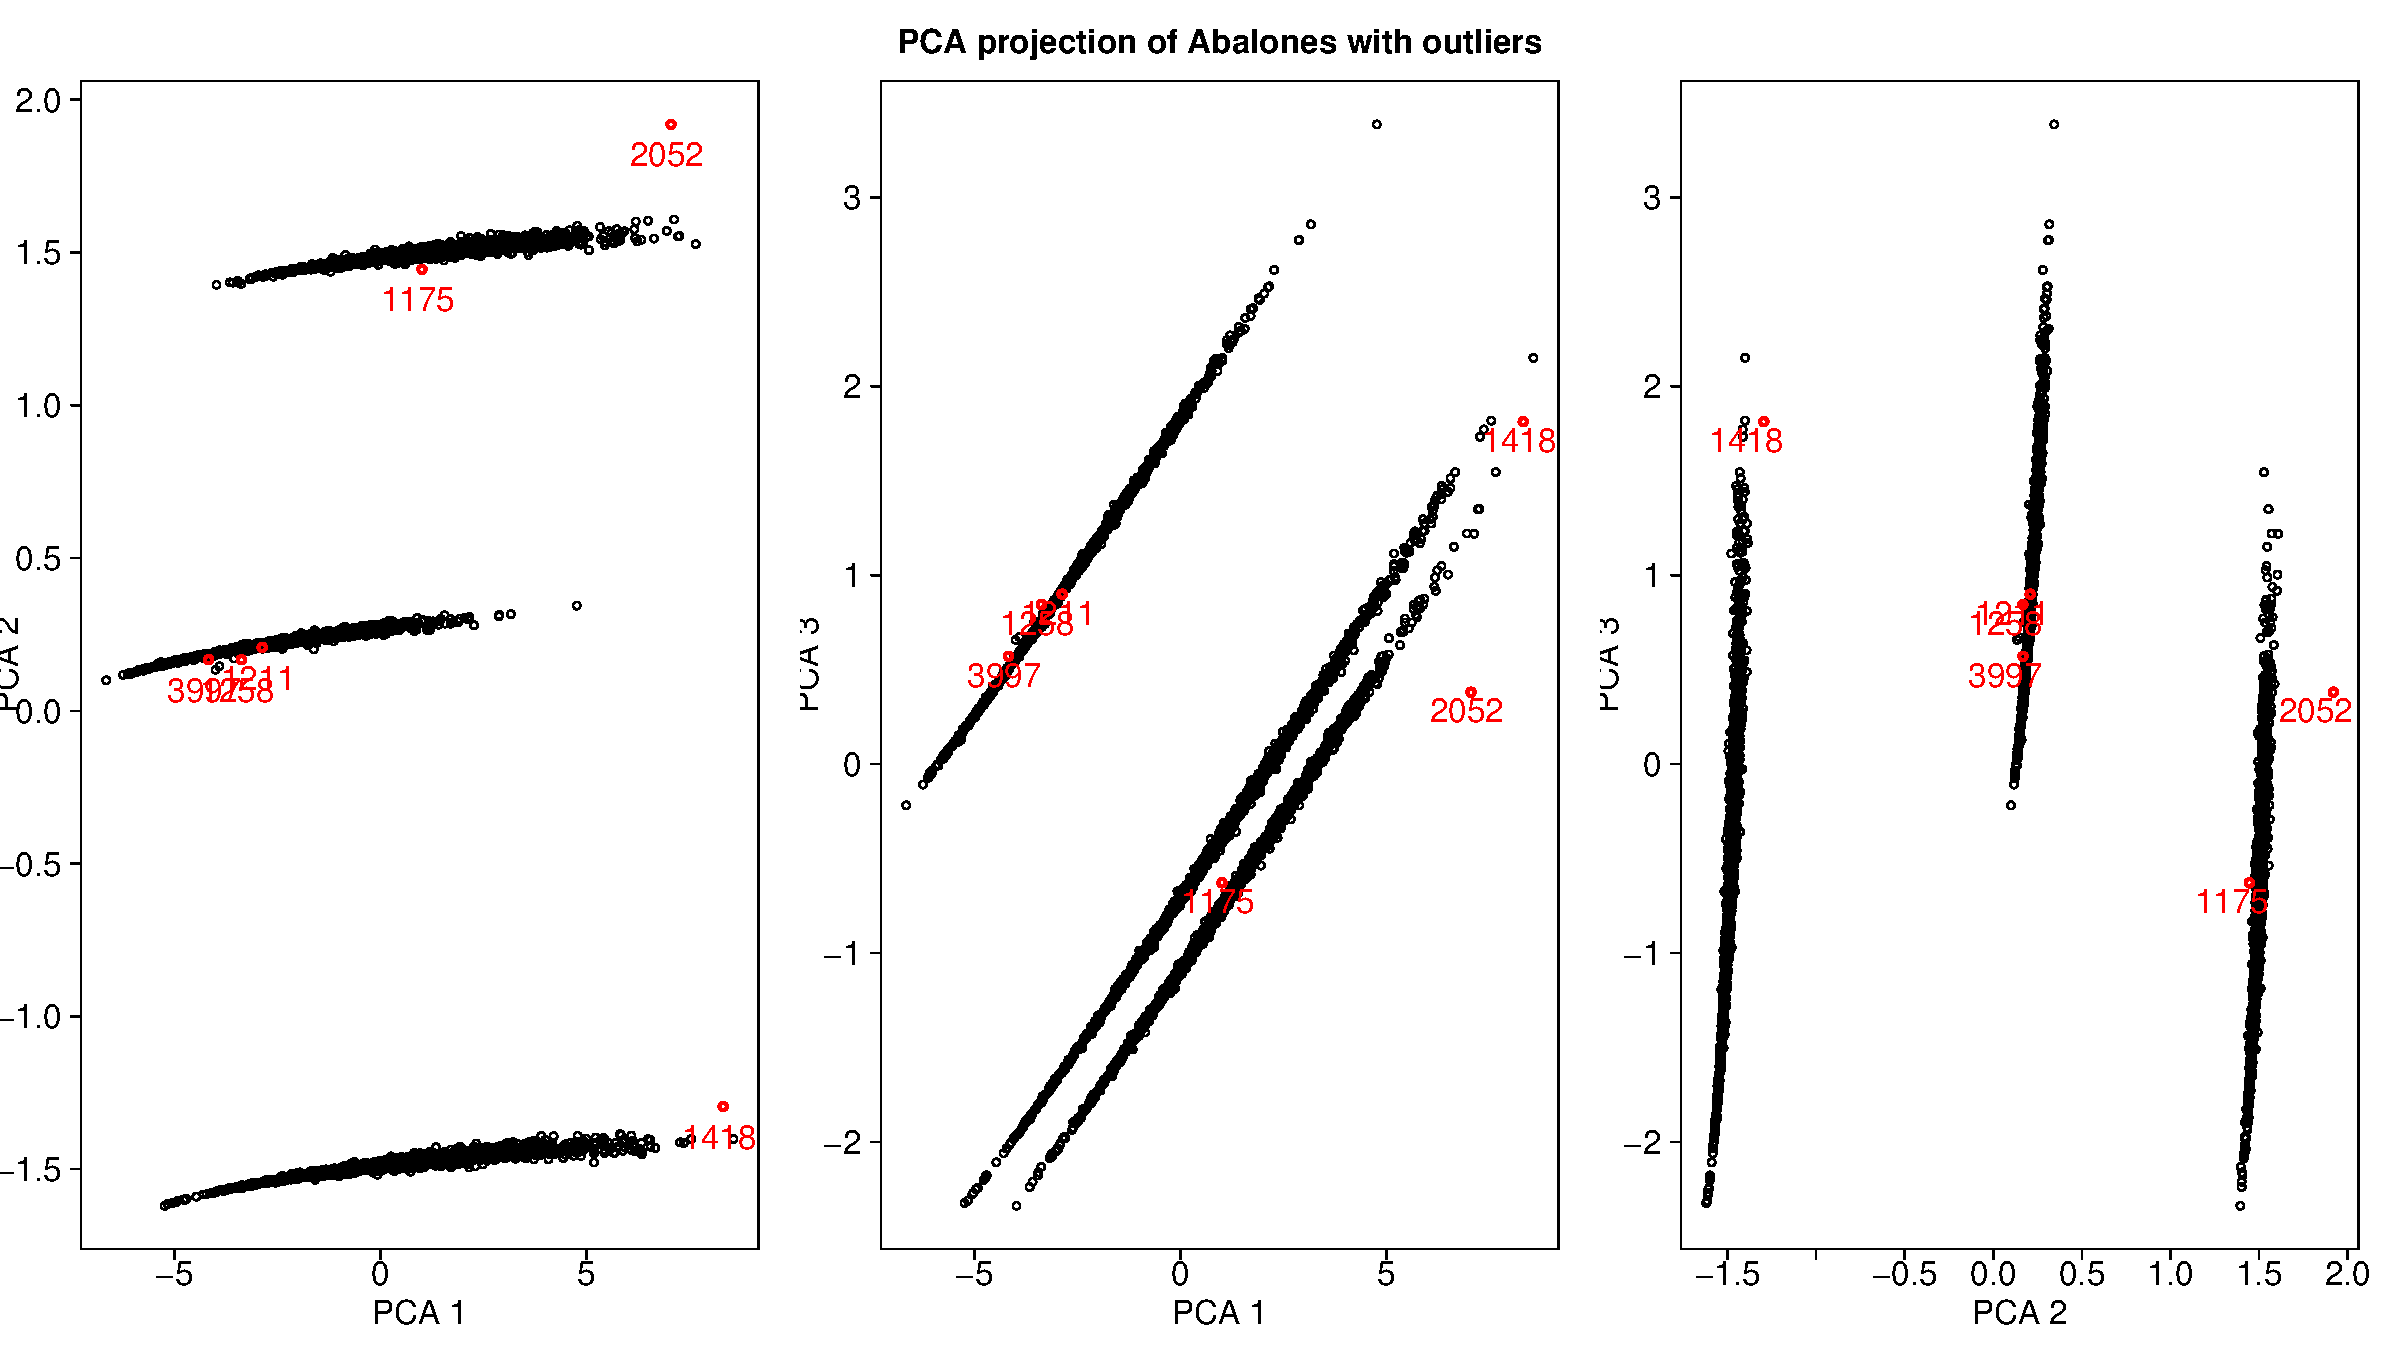
\includegraphics[width = 0.99\textwidth]{data_outliers.pdf}
  \end{minipage} \vfill
  \caption{a) Ranking of observations of the Abalones dataset by GKD, KNND,
    KNNARD, DKNN for k = 30, first 20 observations showed.  b) PCA projection of
    Abalones data on three first principal components with outliers visualized
    as red circles with corresponding index numbers.}
  \label{fig:data_ranking}
\end{figure}

For GKK, KNND, and KNNARD the lower score, the more extreme is the observation,
and vice versa for DKNN, because it is a measure of distance.  On the basis of
the ranking in Fig.~\ref{fig:data_ranking}a, we did the following: we noticed
that for example observation 2052 was ranked first by each of the scoring
methods.  We found all index numbers of the observations, that were ranked as
the first 20 most suspicious by all four scoring methods.  Then, we plotted the
PCA projection of the Abalones dataset with the outliers visualized as red
circles with their index numbers below, and this is presented in
Fig.~\ref{fig:data_ranking}b.  There are six potential outliers visualized on
the first three PCA components, but visually only observations 2052, 1418, and
maybe 1175 deviate significantly from the overall observations in the dataset.
A conservative conclusion would be that there are only two outliers in the
Abalones dataset: observations 1418 and 2052.  Not surprisingly, they correspond
exactly to the observations with anomal height in
Fig.~\ref{fig:data_descriptive_analysis}a:
\begin{verbatim}
> data[1418, ]
Length Diameter   Height  WhlWght ShckdWght VscrWght ShllWght    Male    Female     Infant
1418 1.507232 1.583222 8.977051 2.816657  3.370529 2.790754 1.962384 1.31652 -0.674753 -0.6879355
> data[2052, ]
Length  Diameter   Height    WhlWght  ShckdWght   VscrWght   ShllWght       Male   Female     Infant
2052 -0.5744894 -0.532863 23.68045 -0.4786856 -0.1232976 -0.5892811 -0.7566727 -0.7593967 1.481669 -0.6879355
\end{verbatim}

%%%%%%%%%%%%%%%%%%%% Results and discussion
\section{Results and discussion}
\label{sec:results_and_discussion}
The considered clustering problem was to cluster the Abalones data according to
the age range they belong to.  We considered the equal length grouping of the
Age attribute to label the points, and used GMM and HCA for clustering.  We
found that GMM is not able to detect the optimal number of components in the
model, and therefore we used the number of clusters that equals to the number of
original clusters in the data for the hierarchial clustering.  Comparing the two
methods, we found that their performance is simply the same according to the
used cluster validity measures.

For the association mining, we found that the only age above the median (Age.H) is a frequent itemset. The AR found shown that the abalones age presents a strong relation with the mentioned physical characteristics. Also, no evidence that associate abalones age with their sex were found, indicating that the abalones age can be explained only by their physical characteristics.

As for the anomally detection, we found two extreme observations that correspond
to the abnormally high value of height of abalones, and checked that all the
observation ranking methods indeed ranked those two points as outliers.
%%%%%%%%%%%%%%%%%%%% Bibliography %%%%%%%%%%%%%%%%%%%%
%% \begin{thebibliography}{10}
%% \bibitem{datadescription} \url{http://archive.ics.uci.edu/ml/datasets/Abalone}
%% \bibitem{gam} \url{https://en.wikipedia.org/wiki/Generalized_additive_model}
%% \bibitem{Waugh.thesis} S.~Waugh,''Extending and Benchmark Cascade-Correlation,''
%%   Thesis, 1997.
%% \bibitem{Mayukh} H.~Mayukh, ``Age of Abalones using Physical
%%   Characteristics: A Classification Problem,'' ECE 539 Fall 2010
%%   Project Report, Department of Electrical and Computer Engineering
%%   University of Wisconsin-Madison, 2010.
%% \end{thebibliography}
\end{document}
